\chapter{Sequential Monte Carlo for Bayesian Computation}
\label{cha:Sequential Monte Carlo for Bayesian Computation}

As reviewed in Chapter~\ref{cha:Monte Carlo Methods}, \mcmc algorithms, though
widely used for the purpose of Bayesian computation, have many limitations.
Algorithms such as \rjmcmc are conceptually appealing, yet often difficult to
design in practice. Other algorithms such as the Metropolis-Hastings algorithm
and the Gibbs sampling, though provide generic frameworks, within which
problems in many fields can be solved, the design of efficient, high
performance algorithms still requires considerable expertise and sometimes
extensive experience.

In recent years, there is a tendency of considering population based
algorithms. A common theme in these algorithms is that, instead of simulating
directly from complex target distribution, related yet simpler distributions
are used to ``help'' the simulation. One such algorithm, which is essentially
a generalization of the Metropolis-Hastings algorithm, population \mcmc is
reviewed in Section~\ref{sub:Population mcmc}, in which the easier to simulate
distribution ``lends'' information to the target and accelerates its mixing.
Another example of population based algorithm is the recent development of
particle \mcmc \cite{Andrieu:2010gc}, which embed \smc samplers inside \mcmc
algorithms. The \smc sampler will be the central topic of this chapter

Sequential Monte Carlo (\smc) samplers, in various forms has been around for
more than a decade and widely used in many fields. Until recently there has
been little interest in using it for Bayesian model comparison for a few
reasons. One of the more important one is that, when \mcmc algorithms are
available, \smc could cost more computational resources than a well designed
\mcmc algorithm. However we believe there are at least two important reasons
that \smc can be preferable to \mcmc for the purpose of Bayesian model
comparison. First, it provides a generic and robust framework for simulation
from complex distributions that are difficult for \mcmc algorithms, especially
for high dimensional multimodal distributions. Though it is not impossible to
design \mcmc algorithms for the same problems, it can be hugely difficult in
practice. The \smc framework provides an alternative that is easy to use.  It
has the potential to enable statisticians to construct more realistic, useful
models that were previously difficult to use due to the computational
complexity. Second, most Monte Carlo algorithms has to be implemented on
computers to be useful. Therefore it is unrealistic to not consider the trend
of today's computer technologies, in particular, parallel computing. \smc is
much more suitable for this kind of computing than conventional \mcmc. As we
will see later, \smc has certain advantages over some other parallelized
algorithms.

In this chapter, we first give a review of \smc algorithms in
Section~\ref{sec:Sequential Monte Carlo samplers}. It is followed by a section
that details the use of \smc in the context of Bayesian model comparison.
Next, Section~\ref{sec:Extensions and refinements} develops some extensions
and refinements of existing practices. It is followed by a discussion of how
the presented framework lead to an automatic and generic algorithms. This
chapter is concluded with an extensive empirical performance studies of
various proposed strategies.

\section{Sequential Monte Carlo samplers}
\label{sec:Sequential Monte Carlo samplers}

\smc samplers allow us to obtain, iteratively, collections of weighted samples
from a sequence of distributions $\{\pi_t\}_{t\ge0}$ over essentially any
random variables on some measurable spaces $(E_t,\calE_t)$. It is an extension
of the \emph{sequential importance sampling} (\sis) technique, which is a
generalization of particle filter algorithms widely used in physics and signal
tracking literature. In the remainder of this section, sequential importance
sampling and resampling algorithms are introduced. Then how they are
generalized to \smc samplers for the purpose of the current work are
discussed. To simplify the discussion, we will assume that the distributions
are continuous and their density functions which will also be denoted
by $\{\pi_t\}_{t\ge0}$.

\subsection{Sequential importance sampling and resampling}
\label{sub:Sequential importance sampling and resampling}

Sequential importance sampling (\sis) generalizes the importance sampling (see
Section~\ref{sec:Importance sampling}) technique for a sequence of
distributions $\{\pi_t\}_{t\ge0}$ defined on spaces
$\{\prod_{k=0}^tE_k\}_{t\ge0}$. The algorithm operates as the following.

At time $t = 0$, draw $\{X_0^{(i)}\}_{i=1}^N$ from $\eta_0$ and compute the
weights $W_0^{(i)} \propto \pi_0(X_0^{(i)})/\eta_0(X_0^{(i)})$. At time
$t\ge1$, each sample $X_{0:t-1}^{(i)}$, usually termed \emph{particles} in the
literature, is extended to $X_{0:t}^{(i)}$ by sampling from a proposal
distribution $q_t(\cdot|X_{0:t-1}^{(i)})$. The weights are recalculated as
$W_t^{(i)} \propto \pi_t(X_{0:t}^{(i)})/\eta_t(X_{0:t}^{(i)})$ where
\begin{equation}
  \eta_t(X_{0:t}^{(i)}) =
  \eta_{t-1}(X_{0:t-1}^{(i)})q_t(X_{0:t}^{(i)}|X_{0:t-1}^{(i)})
\end{equation}
and thus
\begin{align}
  W_t^{(i)} \propto \frac{\pi_t(X_{0:t}^{(i)})}{\eta_t(X_{0:t}^{(i)})}
  &= \frac{\pi_t(X_{0:t}^{(i)})\pi_{t-1}(X_{0:t-1}^{(i)})}
  {\eta_{t-1}(X_{0:t-1}^{(i)})q_t(X_{0:t}^{(i)}|X_{0:t-1}^{(i)})
    \pi_{t-1}(X_{0:t-1}^{(i)})} \notag\\
  &= \frac{\pi_t(X_{0:t}^{(i)})}
  {q_t(X_{0:t}^{(i)}|X_{0:t-1}^{(i)})\pi_{t-1}(X_{0:t-1}^{(i)})}W_{t-1}^{(i)}.
  \label{eq:si}
\end{align}
The importance sampling approximation of $\Exp_{\pi_t}[\varphi_t(X_{0:t})]$
can be obtained using $\{W_t^{(i)},X_{0:t}^{(i)}\}_{i=1}^N$, where
$\varphi_t(\cdot)$ is some function of interest.

However, this approach fails as $t$ becomes large. The weights tend to become
concentrated on a few particles as the discrepancy between $\eta_t$ and
$\pi_t$ becomes larger. Resampling techniques are applied such that, a new
particle system $\{\bar{W}_t^{(i)},\bar{X}_{0:t}^{(i)}\}_{i=1}^M$ is obtained
with the property,
\begin{equation}
  \Exp\Square[Big]{\sum_{i=1}^M\bar{W}_t^{(i)}\varphi_t(\bar{X}_{0:t}^{(i)})}
  = \Exp\Square[Big]{\sum_{i=1}^NW_t^{(i)}\varphi_t(X_{0:t}^{(i)})}
  \label{eq:resample}
\end{equation}
where $\varphi_t$ is the function of interest. In other words, the resampling
step does not change the expectation of the estimate. In practice, the
resampling algorithm is usually chosen such that $M = N$ and $\bar{W}^{(i)} =
1/N$ for $i=1,\dots,N$. Resampling can be performed at each iteration $t$ or
adaptively based on some criteria of the discrepancy the distribution of
the particles and the target distribution $\pi_t$, accumulated since the last
time resampling was performed. One popular quantity used to monitor this
discrepancy is \emph{effective sample size} (\ess), introduced by
\cite{Liu:1998iu}, defined as
\begin{equation}
  \ess_t = \frac{1}{\sum_{i=1}^N (W_t^{(i)})^2}
\end{equation}
where $\{W_t^{(i)}\}_{i=1}^N$ are the normalized weights. Resampling can be
performed when $\ess\le \alpha N$ where $\alpha\in[0,1]$.

The common practice of resampling is to replicate particles with large weights
and discard those with small weights. In other words, instead of generating a
random sample $\{\bar{X}_{0:t}^{(i)}\}_{i=1}^N$ directly, a random sample of
integers $\{R_t^{(i)}\}_{i=1}^N$ is generated, such that $R_t^{(i)} \ge 0$ for
$i = 1,\dots,N$ and $\sum_{i=1}^N R_t^{(i)} = N$. Each particle value
$X_{0:t}^{(i)}$ is then replicated $R_t^{(i)}$ times in the new particle
system. The distribution of $\{R_t^{(i)}\}_{i=1}^N$ shall fulfill the
requirement of Equation~\ref{eq:resample}. One such distribution is a
multinomial distribution of size $N$ and weights
$(W_t^{(i)},\dots,W_t^{(N)})$ and the resulting algorithm is called the
\emph{multinomial resampling}. See \cite{Douc:2005wa} for some widely used
resampling algorithms. Here we briefly review some of the most commonly used
algorithms besides multinomial resampling.

\paragraph{Residual resampling} This was introduced in \cite{Liu:1998iu}. In
this approach, for $i = 1,\dots,N$, we have
\begin{equation}
  R_t^{(i)} = \Floor{NW_t^{(i)}} + \bar{R}_t^{(i)}
\end{equation}
where $\Floor{}$ denotes the integer part and $\{R_t^{(i)}\}_{i=1}^N$ are
distributed according to a multinomial distribution with size $N - \bar{N}_t$
and weights $(\bar{W}_t^{(i)},\dots,\bar{W}_t^{(N)})$ with
\begin{align*}
  \bar{N}_t &= \sum_{i=1}^N\Floor{NW_t^{(i)}} \\
  \bar{W}_t^{(i)} &= \frac{NW_t^{(i)} - \Floor{NW_t^{(i)}}}{N - \bar{N}_t}
\end{align*}
It was shown that residual resampling can lead to significant variance
reduction for the importance sampling estimator when compared to the
multinomial resampling \cite{Douc:2005wa}. It is easy to see that, unlike
multinomial resampling, in residual resampling, the replication number
$R_t^{(i)}$ will be no less than $NW_t^{(i)} - 1$. The next two resampling
algorithms also share this property.

\paragraph{Stratified resampling} This can be seen in \cite{Kitagawa:1996vx}.
Let $Q$ denote the generalized inverse of the cumulative distribution of a
multinomial distribution with size $N$ and weights $(W_1,\dots,W_N)$. That is
$Q(x) = i$ for $x\in(\sum_{j=1}^{i-1}W_j,\sum_{j=1}^iW_j]$. The stratified
resampling proceeds by first drawing uniform random variates $U_t^{(i)}$ on
$((i-1)/N, i/N]$ for $i = 1,\dots,N$, and then generate $I_t^{(i)} =
Q(U_t^{(i)})$. The new particles system is formed by
$\{X_{0:t}^{(I_t^{(i)})}\}_{i=1}^N$. This algorithm also results in smaller
variance of the importance sampling estimator than that of the multinomial
resampling \cite{Douc:2005wa}.

\paragraph{Systematic resampling} This was mentioned in \cite{Whitley:1994vx}.
Similar to the stratified resampling, the systematic resampling also uses the
inversion method. However, instead of generating $N$ uniform random variates,
it only generates one uniform random variate $U_t$ from $(0, 1/N]$ and
deterministically set $U_t^{(i)} = (i - 1)/N + U_t$ for $i = 1,\dots,N$.
Though it has the most straightforward implementation among all algorithms
introduced so far, it is more complicated to study the behavior of the
conditional variance of the generated samples. As shown in \cite{Douc:2005wa},
there exists counter-examples that the systematic resampling does not
outperform the multinomial resampling.

\paragraph{Combination of residual and stratified/systematic resampling} Both
the stratified and systematic resampling algorithms can be used together with
the residual resampling. It operates by first compute the integer part and the
residual of $NW_t^{(i)}$ for $i = 1,\dots,N$, and then stratified or
systematic resampling are performed using the residuals as weights. It has the
advantage that the resulting algorithm provide better performance than
each of the algorithms involved here \cite{Douc:2005wa}.

There are other specialized resampling algorithms. The algorithms shown above
have a common drawback. They requires the knowledge of all the weights being
available before the algorithm can proceed. Therefore in some situations the
performance of \smc algorithms can be limited by the fact that the resampling
step cannot be parallelized. Parallelized resampling algorithms is an area
that is actively researched (e.g., \cite{Jun:2011vx}). However, we will not
discuss such specialized algorithms in this work.

\subsection[SMC samplers]{\protect\smc samplers}
\label{sub:SMC Samplers}

\smc samplers generalize the \sis algorithm for a sequence of distributions
$\{\pi_t\}_{t\ge0}$ over essentially any random variables on some spaces
$\{E_t\}_{t\ge0}$, by constructing a sequence of auxiliary distributions
$\{\tilde\pi_t\}_{t\ge0}$ on spaces of increasing dimensions,
\begin{equation}
  \tilde\pi_t(x_{0:t})=\pi_t (x_t) \prod_{s=0}^{t-1} L_s(x_{s+1},x_s),
\end{equation}
where the sequence of Markov kernels $\{L_s\}_{s=0}^{t-1}$, termed
\emph{backward kernels}, is formally arbitrary but critically influences the
estimator variance. See \cite{DelMoral:2006hc} for further details and
guidance on the selection of these kernels (also see Section~\ref{sub:Optimal
  and suboptimal backward kernels}).

Standard sequential importance sampling and resampling algorithms can then be
applied to the sequence of synthetic distributions, $\{\tilde\pi_t\}_{t\ge0}$.
The calculation of the importance weights is straightforward. At time $t-1$,
assume that a set of weighted particles
$\{W_{t-1}^{(i)},X_{0:t-1}^{(i)}\}_{i=1}^N$ approximating $\tilde\pi_{t-1}$ is
available, then at time $t$, the path of each particle is extended with a
Markov kernel say, $K_t(x_{t-1}, x_t)$ and the set of particles
$\{X_{0:t}^{(i)}\}_{i=1}^N$ reach the distribution $\eta_t(x_{0:t}^{(i)}) =
\eta_0(x_0^{(i)})\prod_{k=1}^tK_t(x_{t-1}^{(i)}, x_t^{(i)})$ assuming no
resampling has occurred, where $\eta_0$ is the initial distribution of the
particles. To correct the discrepancy between $\eta_t$ and $\tilde\pi_t$,
equation~\ref{eq:si} is applied and in this case,
\begin{equation}
  W_t^{(i)} \propto \frac{\tilde\pi_t(X_{0:t}^{(i)})}{\eta_t(X_{0:t}^{(i)})}
  = \frac{\pi_t(X_t^{(i)})\prod_{s=0}^{t-1}L_s(X_{s+1}^{(i)}, X_s^{(i)})}
  {\eta_0(X_0^{(i)})\prod_{k=1}^tK_k(X_{k-1}^{(i)},X_k^{(i)})}
  \propto \tilde{w}_t(X_{t-1}^{(i)}, X_t^{(i)})W_{t-1}^{(i)}
\end{equation}
where $\tilde{w}_t$, termed the \emph{incremental weights}, are calculated as,
\begin{equation}
  \tilde{w}_t(X_{t-1}^{(i)},X_t^{(i)}) =
  \frac{\pi_t(X_t^{(i)})L_{t-1}(X_t^{(i)}, X_{t-1}^{(i)})}
  {\pi_{t-1}(X_{t-1}^{(i)})K_t(X_{t-1}^{(i)}, X_t^{(i)})}
\end{equation}
If $\pi_t$ is only known up to a normalizing constant, say $\pi_t(x_t) =
\gamma_t(x_t)/Z_t$, then we can use the \emph{unnormalized} incremental
weights
\begin{equation}
  w_t(X_{t-1}^{(i)},X_t^{(i)}) =
  \frac{\gamma_t(X_t^{(i)})L_{t-1}(X_t^{(i)}, X_{t-1}^{(i)})}
  {\gamma_{t-1}(X_{t-1}^{(i)})K_t(X_{t-1}^{(i)}, X_t^{(i)})}
\end{equation}
for importance sampling. Further, with the \emph{normalized}
weights $\{W_{t-1}^{(i)}\}_{i=1}^N$ of the last generation, we can estimate
the ratio of normalizing constant $Z_t/Z_{t-1}$ by
\begin{equation}
  \frac{\hat{Z}_t}{Z_{t-1}} =
  \sum_{i=1}^N W_{t-1}^{(i)}w_t(X_{t-1}^{(i)},X_t^{(i)})
  \label{eq:ratio normalized}
\end{equation}
Iteratively, the ratio of the normalizing constants between initial
distribution $\pi_0$ and some target $\pi_T$, $T\ge1$ can be estimated. The
incremental weights clearly depend on the choice of the backward kernels. See
\cite{DelMoral:2006hc} and Section~\ref{sub:Optimal and suboptimal backward
  kernels} for details on calculating the incremental weights.

\subsection{Sequence of distributions}
\label{sub:Sequence of distributions}

There are many ways to specify the sequence of distributions. For many
applications, such a sequence arises from the problem setting naturally.

In \cite{Chopin:2002hg}, a data tempering scheme was considered in the context
of Bayesian inference for static parameters. Suppose data $\data =
(y_1,\dots,y_n)$ are available and it is of interest to inference the
posterior distribution of some parameter vector $\theta$, $\pi(\theta|\data)$.
Then one can construct the following sequence of distributions
$\{\pi_t\}_{t=1}^n$,
\begin{equation}
  \pi_t(\theta) = \pi(\theta|y_1,\dots,y_t).
\end{equation}
That is, the data is introduced one by one into the posterior. However, this
scheme can be sensitive to the order of data being introduced. A modification
is to introduce a batch of data at each iteration, also introduced in
\cite{Chopin:2002hg}. How many data points to be incorporated in each
iteration can still be difficult to determine. The more data points introduced
at each step, the more degeneracy (measured by, e.g., \ess) will be induced.
It is natural to consider introducing data such that a constant level of
degeneracy is maintained. It is intuitive to see that with enough data (large
$t$), the addition of the same amount of data will have less influence on the
posterior than when there are only a few data (small $t$) being introduced.
It was shown in \cite{Chopin:2002hg} that, under this assumption, it can be
expected that the number of data points at each step increases geometrically.

Another generic scheme is called the \emph{geometric path}. Given the target
distribution $\pi$ and another distribution $\eta$, which usually has the same
support but heavier tails than that of $\pi$, a sequence of distributions
$\{\pi_t\}_{t=0}^T$ can be constructed,
\begin{equation}
  \pi_t(x) = \pi(x)^{\alpha(t/T)}\eta(x)^{1-\alpha(t/T)}
\end{equation}
where $\alpha:[0,1]\to[0,1]$ is a monotonically increasing mapping with
$\alpha(0) = 0$ and $\alpha(1) = 1$. Some variants of this scheme adapted
particularly for the purpose of Bayesian modeling can be seen in
Section~\ref{sub:smc1: An all-in-one approach} and~\ref{sub:smc2: A
  direct-evidence-calculation approach}. The sequence of distributions moves
smoothly from $\eta$, which is usually easy to sample from or to construct an
efficient proposal distribution for, towards the target distribution $\pi$.
However, this scheme has one important drawback. For a high dimensional target
with many well separated modes, it can be difficult for $\eta$ (or its
proposal distribution) to produce samples within each of all the modes and the
sampler may never reach part of the support of the target distribution $\pi$.
This problem can be partially solved by increase the number of particles.

Despite this limitation, the geometric scheme has a significant advantage as
we will see later (Section~\ref{sub:Optimal and suboptimal backward kernels}
and~\ref{sub:Adaptive specification of distributions}). In short, when
combined with certain transition kernels and backward kernels, it allows easy
computation of the weights using quantities already computed in the last
iteration without actually simulating the samples. Therefore it provides a way
to conduct adaptive sampling at low computational cost.

There are other sequences, which often have particular use for certain
applications. For example, for global optimization of a function $f$, such
that $\int f(x)\intd x <\infty$ (that is, it can be normalized into a density
function), one can simulate from a sequence of distributions,
$\{\pi_t\}_{t\ge0}$, defined by,
\begin{equation}
  \pi_t(x) \propto f(x)^{\alpha(t)}
\end{equation}
where $\alpha:[0,\infty)\to[0,\infty)$ is a monotonically increasing mapping
with $\alpha(t)\to\infty$ as $t\to\infty$. The sequence of distributions will
concentrate more and more around the modes of $f$.

\subsection{Sequence of transition kernels}
\label{sub:Sequence of transition kernels}

It is easy to see that, the optimal proposal kernel is $K_t(x_{t-1}, x_t) =
\pi_t(x_t)$, in the sense of minimizing the Monte Carlo variance of the
importance weights. However, this choice is not possible except for trivial
toy examples. Some sensible alternatives have been proposed in the past.

One approach is to use independent proposals, $K_t(x_{t-1},x_t) =
\mu_t(x_{t-1})$ for some distribution $\mu_t$ at each iteration. Usually,
$\mu_t$ belongs to a family of distributions with parameters determined by
certain statistics of the particle system of the last generation, for example,
a multivariate Normal distribution with the mean vector and the covariance
matrix estimated from current samples. For general use, this can be overly
restrictive and the performance can be difficult to calibrate, especially in
high dimensional problems. In this situation, it is difficult for the
independent proposal to capture the characteristics of the target distribution
without knowing it in advance. And thus it can lead to large variance of
importance weights and poor performance of the sampler.

An important alternative, advocated in \cite{DelMoral:2006hc} is to use \mcmc
kernels targeting $\pi_t$. This strategy is particularly justified if the
sequence of distributions moves smoothly or the kernel is fast mixing. When
the sequence of distributions moves slowly from one to another, that is
$\pi_t$ is not very different from $\pi_{t-1}$, and thus samples from
$\eta_{t-1}$ is a good approximation to $\pi_t$, the kernel is likely to
successfully move particles towards high probability regions of $\pi_t$. What
makes it more attractive is the fact that we can use the vast literature on
the design of efficient \mcmc algorithms to build the proposal distributions.
In addition, as we will see very soon, when combined with certain backward
kernels, this approach enables us to calculate the importance weights without
actually simulating samples. And therefore it leads to low computational cost
adaptive algorithms that can improve the performance considerably.

\subsection{Optimal and suboptimal backward kernels}
\label{sub:Optimal and suboptimal backward kernels}

The sequence of backward kernels $\{L_t\}_{t=0}^{T-1}$ should be optimized
with respect to the sequence of transition kernel $\{K_t\}_{t=0}^T$. Let
$\eta_t(x_t)$ denote the marginal distribution of $X_t$. That is,
\begin{equation}
  \eta_t(x_t) = \eta_0(x_0)\prod_{k=1}^tK_k(x_{k-1},x_k)
\end{equation}
if no resampling has occurred and,
\begin{equation}
  \eta_t(x_t) = \pi_l(x_l)\prod_{k=l+1}^tK_k(x_{k-1},x_k)
\end{equation}
if the last resampling occurs at time $l$.

As shown in Proposition~1{} in \cite{DelMoral:2006hc}, the backward kernel
$L_{t-1}(x_t, x_{t-1})$ that minimizes the variance of unnormalized importance
weights is given by,
\begin{equation}
  L_{t-1}^{\opt}(x_t,x_{t-1}) =
  \frac{\eta_{t-1}(x_{t-1})K_t(x_{t-1},x_t)}{\eta_t(x_t)}
\end{equation}
and in this case the weights are,
\begin{equation}
  W_t(X_{t-1},X_t) \propto \frac{\pi_t(X_t)}{\eta_t(X_t)}
\end{equation}
The marginal $\eta_t(x_t)$ is typically not available and thus the above
optimal backward kernel cannot be used in practice.

One sensible alternative is to substitute $\pi_{t-1}$ for $\eta_{t-1}$, that
is,
\begin{equation}
  L_{t-1}(x_t,x_{t-1}) =
  \frac{\pi_{t-1}(x_{t-1})K_t(x_{t-1},x_t)}
  {\int \pi_{t-1}(x_{t-1})K_t(x_{t-1},x_t)\intd x_{t-1}}
  \label{eq:subopt back kernel}
\end{equation}
This approach is justified if the particle system has has been resampled at
time $t-1$, in which case $\eta_{t-1}$ is indeed equal to $\pi_{t-1}$ or when
resampling was at least performed occasionally such that the degeneracy
between $\eta_{t-1}$ and $\pi_{t-1}$ is controlled. The incremental weights
can be computed if the integration above can be computed. Usually this is done
through the unnormalized distribution $\gamma_{t-1}$ instead of $\pi_{t-1}$.
When $\gamma_{t-1}$ is known analytically, the unnormalized incremental
weights are,
\begin{equation}
  w_t(X_{t-1}^{(i)},X_t^{(i)}) =
  \frac{\gamma_t(X_t^{(i)})}
  {\int\gamma_{t-1}(x_{t-1})K_t(x_{t-1},X_t^{(i)})\intd x_{t-1}}.
  \label{eq:inc weight subopt}
\end{equation}
The requirement of the knowledge of the above integration can limit the use of
the kernel in some applications.

When using a \mcmc kernel $K_t$ that is invariant to $\pi_t$ as the
transition kernel, and when $\pi_{t-1}\approx\pi_t$, by substitute $\pi_t$
for $\pi_{t-1}$, Equation~\eqref{eq:subopt back kernel} becomes,
\begin{align}
  L_{t-1}(x_t,x_{t-1})
  &= \frac{\pi_t(x_{t-1})K_t(x_{t-1},x_t)}
  {\int \pi_t(x_{t-1})K_t(x_{t-1},x_t)\intd x_{t-1}} \notag\\
  &= \frac{\pi_t(x_{t-1})K_t(x_{t-1},x_t)}{\pi_t(x_t)}
  \label{eq:subopt back kernel mcmc}
\end{align}
where the second equation is due to the fact that $K_t$ is invariant to
$\pi_t$. It is easy to see that the unnormalized incremental weights are,
\begin{equation}
  w_t(X_{t-1}^{(i)},X_t^{(i)}) =
  \frac{\gamma_t(X_{t-1}^{(i)})}{\gamma_{t-1}(X_{t-1}^{(i)})}.
  \label{eq:inc weight subopt mcmc}
\end{equation}
Note that, the incremental weights no longer depend on the samples from
iteration $t$, $\{X_t^{(i)}\}$. Therefore, it can be calculated before the
sampling step, which moves the particles according to the kernel $K_t$. Since
the incremental weights solely depends on the specification of $\gamma_t$,
which usually can be computed point-wise, given the current samples, it is
possible to specify $\gamma_t$ (and therefore $\pi_t$) according to the
calculated weights using informations from the current samples before carrying
out the actual simulation of the current iteration.

However the expression~\eqref{eq:inc weight subopt mcmc} is not without
drawbacks. Compared to the expression~\eqref{eq:inc weight subopt}, which is
more intuitive since it considers the transition kernel $K_t$, which depends
on the current samples, it benefits less from fast mixing kernels. If $\pi_t$
is not close to $\pi_{t-1}$, then the variance of the incremental weights is
likely to be large even the kernel $K_t$ mixes fast. Indeed, later we will
show empirically that, it is preferable to use more distributions rather than
using multiple passes of \mcmc moves in a single iteration, provided that they
use the same computational resources.

\section{Application to Bayesian model comparison}
\label{sec:Application to Bayesian model comparison}

The application of \smc samplers to Bayesian model comparison is
straightforward. However, it has been overlooked in recent years. In this
section, we outline common strategies of using \smc samplers for Bayesian
model comparison. In the next section, we introduce some innovative refinement
and extensions to existing practices.

As reviewed in Section~\ref{sub:Model choice problems}, The problem of
interest is characterizing the posterior distribution over
$\{\calM_k\}_{k\in\calK}$, a set of possible models, with model $\calM_k$
having parameter vector $\theta_k\in\Theta_k$ which must also usually be
inferred. Given prior distributions $\pi(\calM_k)$ and $\pi(\theta_k|\calM_k)$
and the likelihood function $p(\data|\theta_k,\calM_k)$, we seek the posterior
distributions $\pi(\calM_k|\data)\propto p(\data|\calM_k)\pi(\calM_k)$. There
are three fundamentally different approaches to the computations,
\begin{enumerate}
  \item Calculate posterior model probability distribution
    $\pi(\calM_k|\data)$ directly.
  \item Calculate the evidence, the marginal likelihood $p(\data|\calM_k)$, of
    each model.
  \item Calculate pairwise evidence ratios, the Bayes factor $B_{12} =
    p(\data|\calM_{k_1})/p(\data|\calM_{k_2})$ for two models indexed by $k_1$
    and $k_2$.
\end{enumerate}
Each approach admits a natural \smc strategy.

\subsection[SMC1: An all-in-on approach]{\smc[1]: An all-in-one approach}
\label{sub:smc1: An all-in-one approach}

One could consider obtaining samples from the same distribution employed in
the \rjmcmc (see Section~\ref{sub:Reversible jump mcmc}) approach to model
comparison, namely,
\begin{equation}
  \pi^{(1)}(\calM_k,\theta_k) \propto
  \pi(\calM_k)\pi(\theta_k|\calM_k)p(\data|\theta_k,\calM_k)
\end{equation}
which is defined on the disjoint union space
$\bigcup_{k\in\calK}(\{\calM_k\}\times\Theta_k)$.

One obvious \smc approach is to define a sequence of distributions
$\{\pi_t^{(1)}\}_{t=0}^T$ such that $\pi^{(1)}_0$ is easy to sample from,
$\pi_{T}^{(1)} = \pi^{(1)}$ and the intermediate distributions move smoothly
between them. In the remainder of this section, we use the notation
$(\calM_t,\theta_t)$ to denote a random sample on the space
$\bigcup_{k\in\calK}(\{\calM_k\}\times\Theta_k)$ at time $t$. One simple
approach, which might be expected to work well, is the use of an annealing
scheme such that,
\begin{equation}
  \pi^{(1)}_t(\calM_t,\theta_t) \propto \pi(\calM_t)\pi(\theta_t|\calM_t)
  p(\data|\theta_t,\calM_t)^{\alpha(t/T)},
  \label{eq:geometry_1}
\end{equation}
for some monotonically increasing $\alpha:[0,1]\to[0,1]$ such that $\alpha(0)
= 0$ and $\alpha(1) = 1$. Other approaches are possible and might prove more
efficient for some problems (such as the ``data tempering'' approach which
\cite{Chopin:2002hg} proposed for parameter estimation which could easily
be incorporated in our framework), but this strategy provides a convenient
generic approach. These choices lead to Algorithm~\ref{alg:smc1}.

\begin{algorithm}
\begin{algorithmic}
  \tophrule
  \STATE \emph{Initialisation:} Set $t\leftarrow0$.
  \STATE\STATESKIP Sample $X_0^{(i)} = (\theta_0^{(i)},\calM_0^{(i)})\sim\nu$
  for some proposal distribution $\nu$ (usually the joint prior).
  \STATE\STATESKIP Weight $W_0^{(i)} \propto w_0(X_0^{(i)}) =
  {\pi(\calM_0^{(i)}) \pi(\theta^{(i)}_0|\calM_0^{(i)})}/
  {\nu(\theta_0^{(i)},\calM_0^{(i)})}$.
  \STATE\STATESKIP Apply resampling if necessary (e.g., if \ess less than some
  threshold; see Section~\ref{sub:Sequential importance sampling and
    resampling}).

  \STATE \emph{Iteration:} Set $t\leftarrow t + 1$.
  \STATE\STATESKIP Weight $W_t^{(i)} \propto W_{t-1}^{(i)}
  p(\data|\theta_{t-1}^{(i)},\calM_{t-1}^{(i)})^{\alpha(t/T) - \alpha([t-1]/T)}$.
  \STATE\STATESKIP Apply resampling if necessary.
  \STATE\STATESKIP Sample $X_t^{(i)} \sim K_t(\cdot|X_{t-1}^{(i)})$, a
  $\pi_t^{(1)}$-invariant kernel.

  \STATE \emph{Repeat} the \emph{Iteration} step \emph{until $t = T$}.
  \bottomhrule
\end{algorithmic}
\caption{\smc[1]: An All-in-One Approach to Model Comparison.}
\label{alg:smc1}
\end{algorithm}


This approach might outperform \rjmcmc when it is difficult to design
fast-mixing Markov kernels. There are many examples of such an annealed \smc
strategy outperforming \mcmc at a given computational cost -- see, for
example, \cite{Fan:2008tf,Johansen:2008kp,Fearnhead:2010ua}. Such
trans-dimensional \smc has been proposed in several contexts such as
\cite{Peters:2005wh}, and an extension was proposed and analyzed by
\cite{Jasra:2008bb}.

We include this approach for completeness and study it empirically later.
However, the more direct approaches described in the following sections lead
more naturally to easy-to-implement strategies with good performance.

\subsection[SMC2: A direct-evidence-calculation approach]
{\smc[2]: A direct-evidence-calculation approach}
\label{sub:smc2: A direct-evidence-calculation approach}

An alternative approach would be to estimate explicitly the evidence
associated with each model. We propose to do this by sampling from a sequence
of distributions for each model, starting from the parameter prior and
sweeping through a sequence of distributions to the posterior.

Numerous strategies are possible to construct such a sequence of
distributions, but one option is to use for each model $\calM_k$, $k\in\calK$,
the sequence $\{\pi_t^{(2,k)}\}_{t=0}^{T_k}$, defined by
\begin{equation}
  \pi_t^{(2,k)}(\theta_t) \propto
  \pi(\theta_t|\calM_k)p(\data|\theta_t,\calM_k)^{\alpha_k(t/T_k)}.
  \label{eq:geometry_2}
\end{equation}
where the number of distributions, $T_k$, and the annealing schedule,
$\alpha_k:[0,1]\to[0,1]$, may be different for each model. This leads to
Algorithm~\ref{alg:smc2}.

\begin{algorithm}
\begin{algorithmic}
  \tophrule
  \STATE For each model $k \in \calK$ perform the following algorithm.

  \STATE \emph{Initialisation:} Set $t\leftarrow0$.
  \STATE\STATESKIP Sample $\theta_0^{(k,i)}\sim\nu_k$ for some proposal
  distribution $\nu_k$ (usually the parameter prior).
  \STATE\STATESKIP Weight $W_0^{(k,i)} \propto w_0(\theta_0^{(k,i)}) =
  {\pi(\theta_0^{(k,i)}|\calM_k)}/{\nu_k(\theta_0^{(k,i)})}$.
  \STATE\STATESKIP Apply resampling if necessary.

  \STATE \emph{Iteration:} Set $t\leftarrow t + 1$.
  \STATE\STATESKIP Weight $W_t^{(k,i)} \propto W_{t-1}^{(k,i)}
  p(\data|\theta_{t-1}^{(k,i)},\calM_k)^{\alpha_k(t/T_k)-\alpha_k([t-1]/T_k)}$.
  \STATE\STATESKIP Apply resampling if necessary.
  \STATE\STATESKIP Sample $\theta_t^{(k,i)} \sim
  K_t(\cdot|\theta_{t-1}^{(k,i)})$, a $\pi_t^{(k,2)}$-invariant kernel.

  \STATE \emph{Repeat} the \emph{Iteration} step \emph{until $t = T_k$}.
  \bottomhrule
\end{algorithmic}
\caption{\smc[2]: A Direct-Evidence-Calculation Approach.}\label{alg:smc2}
\end{algorithm}


The estimator of the posterior model probabilities depends upon the approach
taken to estimate the normalizing constant. Direct estimation of the evidence
can be performed using the output of this \smc algorithm and the standard
estimator, termed \smc[2]-\ds below (see also Equation~\eqref{eq:ratio
  normalized}), is given by,
\begin{equation}
  \sum_{i=1}^N \frac{\pi(\theta_0^{(k,i)}|\calM_k)}{\nu_k(\theta_0^{(k,i)})}
  \times \prod_{t=2}^T \sum_{i=1}^N W_{t-1}^{(k,i)}
  p(\data|\theta_{t-1}^{(k,i)},\calM_k)^{\alpha_k(t/T_k) - \alpha_k([t-1]/T_k)}
  \label{eq:smc2-ds}
\end{equation}
where $W_{t-1}^{(k,i)}$ is the normalized importance weights of particle $i$,
$\theta_{t-1}^{(k,i)}$, during iteration $t-1$ for model $\calM_k$. An
alternative approach to computing the evidence is also worthy of
consideration. As has been suggested, and shown to perform well empirically
previously \cite{Johansen:2006wm}, it is possible to use all
of the samples from every generation of an \smc sampler to approximate the
path sampling estimator and hence to obtain an estimate of the ratio of
normalizing constants. Section~\ref{sub:Path Sampling via smc2/smc3} provides
details for the use of path sampling for both this and other \smc algorithms
discussed later.

The posterior distribution of the parameters conditional upon a particular
model can also be approximated with,
\begin{equation*}
  \hat{\pi}_{T_k}^{(2,k)}(\diff\theta) =
  \sum\limits_{i=1}^{N} W_{T_k}^{(k,i)}
  \delta_{\theta^{(k,i)}_{T_k}}(\diff\theta).
\end{equation*}
where $\delta_{\theta^{(k,i)}_{T_k}}$ is the Dirac measure.

This approach is appealing for several reasons. One is that it is designed to
estimate directly the quantity of interest: the evidence, producing samples
from that distribution at the same time. Another advantage of this approach
over \smc[1] and the \rjmcmc is that it provides as good a characterization of
each model as is required: it is possible to obtain a good estimate of the
parameters of every model, even those for which the posterior probability is
small. Perhaps most significant is the fact that this approach does not
require the design of proposal distributions or Markov kernels which move from
one model to another: each model is dealt with in isolation. Whilst this may
not be desirable in every situation, there are circumstances in which
efficient moves between models are almost impossible to devise.

This approach also has some disadvantages. In particular, it is necessary to
run a separate simulation for each model -- rendering it impossible to deal
with countable collections of models (although this is not such a substantial
problem in many interesting cases). The ease of implementation may often
offset this limitation.

\subsection[SMC3: A relative-evidence-calculation approach]
{\smc[3]: A relative-evidence-calculation approach}
\label{sub:smc3: A relative-evidence-calculation approach}

A final approach can be thought of as \emph{sequential model comparison}.
Rather than estimating the evidence associated with any particular model, we
could estimate pairwise evidence ratios directly. The \smc sampler starts with
a initial distribution being the posterior of one model (which could comes
from a separate \smc sampler starting from its prior) and moves towards the
posterior of another related model. Then the sampler can continue towards
another related model.

Given a finite collection of models $\{\calM_k\}$, $k\in\calK$, suppose the
models are ordered in a sensible way (e.g., $\calM_{k-1}$ is nested within
$\calM_k$ or $\theta_k$ is of higher dimension than $\theta_{k-1}$). For each
$k\in\calK$, we consider a sequence of distributions
$\{\pi_t^{(3,k)}\}_{t=0}^{T_k}$, such that,
\begin{align*}
  \pi_0^{(3,k)}(\calM,\theta) &=
  \pi(\theta|\data,\calM_k) \bbI_{\{\calM_k\}}(\calM) \\
  \pi_{T_k}^{(3,k)}(\calM,\theta) &=
  \pi(\theta|\data,\calM_{k+1})
  \bbI_{\{\calM_{k+1}\}}(\calM) = \pi_{0}^{(3,k+1)}(\calM,\theta).
\end{align*}
When it is possible to construct an \smc sampler that iterates over this
sequence of distributions, the estimate of the ratio of normalizing constants
is the Bayes factor estimate of model $\calM_{k+1}$ in favor of model
$\calM_k$.

This approach is conceptually appealing, but requires the construction of a
smooth path between the posterior distributions of interest. The geometric
annealing strategy which has been advocated as a good generic strategy in the
previous sections is only appropriate when the support of successive
distributions is non-increasing. This is unlikely to be the case in
interesting model comparison problems.

Here we consider a sequence of distributions on the disjoint union space
$\{\calM_k,\Theta_k\}\cup\{\calM_{k+1},\Theta_{k+1}\},$ with the sequence of
distributions $\{\pi_t^{(3,k)}\}_{t=0}^{T_k}$ defined as the full posterior,
\begin{equation}
  \pi_t^{(3,k)}(\calM_t,\theta_t) \propto
  \pi_t(\calM_t) \pi(\theta_t|\calM_t) p(\data|\theta_t,\calM_t)
\end{equation}
where $\calM_t\in\{\calM_k,\calM_{k+1}\}$ and the prior of models at time $t$,
$\pi_t(\calM_t)$ is defined by
\begin{equation}
  \pi_t(\calM_{k+1}) = \alpha_k(t/T_k)
  \label{eq:smc3_prior}
\end{equation}
for some monotonically increasing $\alpha_k:[0,1]\to[0,1]$ such that
$\alpha_k(0) = 0$ and $\alpha_k(1) = 1$. It is clear that the \mcmc moves
between iterations need to be similar to those in the \rjmcmc or \smc[1]
algorithms. The difference is that instead of efficient exploration of the
whole model space, only moves between two models are required and the sequence
of distributions employed helps to ensure exploration of both model spaces.
The algorithm for this particular sequence of distributions is outlined in
Algorithm~\ref{alg:smc3}. It can be extended to other possible sequence of
distributions between models.

\begin{algorithm}
\begin{algorithmic}
  \tophrule
  \STATE \emph{Initialisation:} Set $k\leftarrow1$.
  \STATE\STATESKIP Use Algorithm~\ref{alg:smc2} to obtain weighted samples
  for $\pi_{T_1}^{(3,1)}$, the parameter posterior for model $\calM_1$

  \STATE \emph{Relative Evidence Calculation}
  \STATE\STATESKIP Set $k\leftarrow k + 1$, $t\leftarrow0$.
  \STATE\STATESKIP Let
  $\{W_0^{(k,i)},X_0^{(k,i)}\}_{i=1}^N$ where $X_0^{(k,i)} =
  (\theta_0^{(k,i)},\calM_0^{(k,i)})$ denote the current samples.
  \STATE\STATESKIP Apply resampling if necessary.

  \STATE\STATESKIP \emph{Iteration:} Set $t\leftarrow t + 1$.
  \STATE\STATESKIP\STATESKIP Weight $W_t^{(k,i)} \propto W_{t-1}^{(k,i)}
  {\pi_t(\calM_{t-1}^{(k,i)})}/{\pi_{t-1}(\calM_{t-1}^{(k,i)})}$.
  \STATE\STATESKIP\STATESKIP Apply resampling if necessary.
  \STATE\STATESKIP\STATESKIP Sample $(\theta_t^{(k,i)},\calM_t^{(k,i)}) \sim
  K_t(\cdot|\theta_{t-1}^{(k,i)},\calM_{t-1}^{(k,i)})$, a
  $\pi_t^{(3,k)}$-invariant kernel.

  \STATE\STATESKIP \emph{Repeat the \emph{Iteration} step up to $t = T_k$}.

  \STATE \emph{Repeat} the \emph{Relative Evidence Calculation} step \emph{until
    sequentially all relative evidences are calculated}.
  \bottomhrule
\end{algorithmic}
\caption{\smc[3]: A Relative-Evidence-Calculation Approach to Model Comparison.}
\label{alg:smc3}
\end{algorithm}


An advantage of this approach is that it provides direct estimate of the Bayes
factor which is of interest for model comparison purpose while not requiring
exploration of as complicated a space as that employed within \rjmcmc or
\smc[1]. The estimator of normalizing constant in \smc[3] follows in
exactly the same manner as in the \smc[2] case. In \smc[3], the same estimator
provides a direct estimate of the Bayes factor.

\subsection{Path Sampling via \smc[2]/\smc[3]}
\label{sub:Path Sampling via smc2/smc3}

The estimation of the normalizing constant associated with our sequences of
distributions can be achieved by a Monte Carlo approximation to the \emph{path
  sampling} formulation given by \cite{Gelman:1998ei}. This is similar to the
technique for population \mcmc as described in Section~\ref{sub:MCMC
  Application to Bayesian model comparison}. In the context of \smc, this
approach is also very closely related to the use of \ais for the same purpose
\cite{Neal:2001we} but as will be demonstrated below the incorporation of some
other elements of more general \smc algorithms can improve performance at
negligible cost. Recall that, given a parameter $\alpha$ which defines a
family of distributions, $\{\pi_{\alpha} = \gamma_{\alpha} / Z_\alpha\}_{\alpha \in
  [0,1]}$ which move smoothly from $\pi_0 = \gamma_0 / Z_0$ to $\pi_1 =
\gamma_1 / Z_1$ as $\alpha$ increases from zero to one, one can estimate the
logarithm of the ratio of their normalizing constants via a simple integral
relationship which holds under very mild regularity conditions,
\begin{equation*}
  \log\Round[bigg]{\frac{Z_1}{Z_0}} =
  \int_{0}^{1} \Exp_{\pi_\alpha} \Square[bigg]{
    \frac{\diff\log\gamma_{\alpha}(X)}{\diff\alpha}
  } \intd\alpha,
\end{equation*}
where the inner expectation is taken with respect to $\pi_{\alpha}$. Note that
the sequence of distributions in the \smc[2] and \smc[3] algorithms above, can
both be interpreted as belonging to such a family of distributions, with
$\alpha = \alpha_k(t/T_k)$, where the mapping $\alpha_k:[0,1]\to[0,1]$ is
again monotonically increasing with $\alpha_k(0) = 0$ and $\alpha_k(1) = 1$.

The \smc sampler provides us with a set of weighted samples obtained from a
sequence of distributions suitable for approximating this integral. At each
$t$ we can obtain an estimate of the expectation within the integral for
$\alpha = \alpha_k(t/T)$ via the usual importance sampling estimator, and this
integral can then be approximated via numerical integration. Whenever the
sequence of distributions employed by \smc[3] has appropriate
differentiability it is also possible to employ path sampling to estimate,
directly, the Bayes factor via this approach applied to the samples generated
by that algorithm. In general, given an increasing sequence
$\{\alpha_t\}_{t=0}^T$ where $\alpha_0 = 0$ and $\alpha_T = 1$, a family of
distributions $\{\pi_{\alpha}\}_{\alpha\in[0,1]}$ as before, and an \smc
sampler that iterates over the sequence of distribution $\{\pi_t =
\pi_{\alpha_t} = \gamma_{\alpha_t}/Z_{\alpha_t}\}_{t=0}^T$, then with the
weighted samples $\{W_t^{(i)},X_t^{(i)}\}_{i=1}^N$, and $t = 0,\dots,T$, a
path sampling estimator of the ratio of normalizing constants $\Xi_T =
\log(Z_1/Z_0)$ can be approximated (using an elementary trapezoidal scheme) by
\begin{equation}
  \hat\Xi_{T}^{N} = \sum_{t=1}^T
  \frac{1}{2}(\alpha_t - \alpha_{t - 1})(U_t^N + U_{t-1}^N),
  \label{eq:path_est}
\end{equation}
where
\begin{equation}
  U_t^N = \sum_{i=1}^N
  W_t^{(i)} \frac{\diff\log\gamma_{\alpha}(X_t^{(i)})}{\diff\alpha}
  \Bigm|_{\alpha = \alpha_t}.
\end{equation}

We term these estimators \smc[2]-\ps and \smc[3]-\ps in the followings. The
combination of \smc and path sampling is somewhat natural and has been
proposed before, e.g., \cite{Johansen:2006wm} although not there in a Bayesian
context. Despite the good performance observed in the setting of rare
event simulation, the estimation of normalizing constants by this approach
seems to have received little attention in the literature. We suspect that
this is because of widespread acceptance of the suggestion of
\cite{DelMoral:2006hc}, that \smc doesn't outperform \ais when normalizing
constants are the object of inference or that of \cite{Calderhead:2009bd}
that all simulation-based estimators based around path sampling can be
expected to behave similarly. We will demonstrate below that these
observations, whilst true in certain contexts, do not hold in full generality.

\section{Extensions and refinements}
\label{sec:Extensions and refinements}

The algorithms introduced in the last section can be seen as straightforward
application of the well established \smc algorithms to Bayesian model
comparison. Though by construction, \smc algorithms can be more robust than
many \mcmc and other algorithms. However, as with any Monte Carlo algorithms,
without careful design, the performance can be far from satisfactory for
realistic applications. In this section, we introduce some extensions and
refinement that can further improve the presented framework. Of course, they
cannot guarantee that the algorithms will perform well for all possible
situations. However, it provide robust and reliable solutions for many
realistic applications with minimal manual tuning. For more difficult
problems, they also provide a solid foundation on top of which algorithms with
higher performance can be built.

We will use the \pet compartmental model example for illustrative purpose in
this section. More comprehensive performance comparisons can be found in
Section~\ref{sec:Performance comparison}. We will consider both simulated and
real data. The simulated data set is the same as in
Chapter~\ref{cha:Introduction}. Due to the large amount of the real data, it
is beyond the resources we have to perform repeated simulations for a whole
\pet scan. Instead, 20 real data sets are sampled from typical region of
interest in a single \pet scan. Figure~\ref{fig:typical real pet} shows three
of them. As we can see, they vary considerably in characteristics despite all
can be described as ``typical'' \pet data. The purpose of the current work is
to advocate robust and self-tuning algorithms. And the variability in the data
sets provides excellent test examples. In addition, in this section, the
models are configured with the non-informative priors without ordering (see
Section~\ref{sub:Choice of priors}) and thus the parameters are exchangeable,
similar to that of a mixture model. This creates a multimodal posterior
surface for models with two or more compartments.

\begin{figure}[t]
  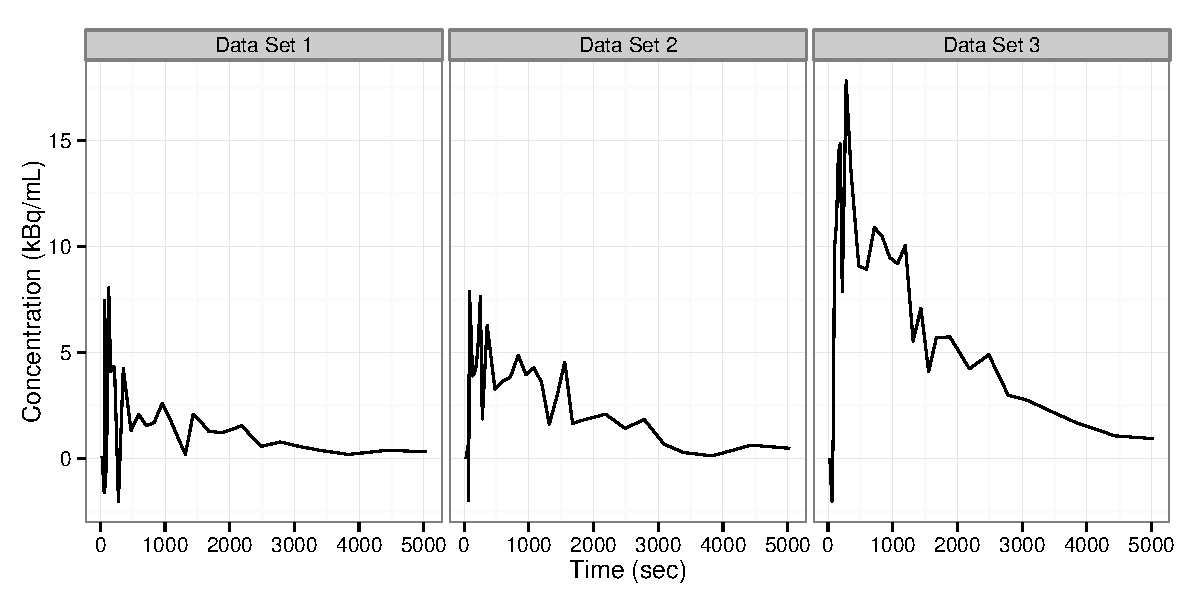
\includegraphics[width=\linewidth]{fig/Typical_PET}
  \caption{Typical real \protect\pet data}
  \label{fig:typical real pet}
\end{figure}

\subsection{Improved univariate numerical integration}
\label{sub:Improved univariate numerical integration}

As seen in the last section, the path sampling estimator requires evaluation
of the expectation,
\begin{equation*}
  \Exp_{\pi_\alpha}\Square[bigg]{
    \frac{\diff\log\gamma_{\alpha}(X)}{\diff\alpha}}
\end{equation*}
for $\alpha\in[0,1]$, which can be approximated by importance sampling using
samples generated by an \smc sampler operating on the sequence of
distributions $\{\pi_t = \pi_{\alpha_t} = \gamma_{\alpha_t}/Z_t\}_{t=0}^T$
directly for $\alpha\in\{\alpha_t\}_{t=0}^T$. For arbitrary $\alpha\in[0,1]$,
finding $t$ such that $\alpha\in(\alpha_{t-1},\alpha_t)$, the expectation can
be easily approximated using existing \smc samples -- the quantities required
in the importance weights to obtain such an estimate have already been
calculated during the running of the \smc algorithm and such computations have
little computational cost.

As noted by \cite{Friel:2012}  we can use more sophisticated numerical
integration strategies to reduce the path sampling estimator bias. For
example, higher order Newton-Cotes rules rather than the Trapezoidal rule can
be implemented straightforwardly. In the case of \smc it is especially
straightforward to estimate the required expectations at arbitrary $\alpha$
and so we cheaply use higher order integration schemes and we can also use
numerical integrations which make use of a finer mesh
$\{\alpha_t'\}_{t=0}^{T'}$ than $\{\alpha_t\}_{t=0}^T$. Since higher order
numerical integrations based on approximations of derivatives obtained from
Monte Carlo methods may potentially be unstable in some situations, the second
approach can be more appealing in some applications. A demonstration of the
bias reduction effect is provided in Section~\ref{sub:Positron Emission
  Tomography compartmental model}.

\subsection{Adaptive specification of distributions}
\label{sub:Adaptive specification of distributions}

In settings in which the importance weights at time $t$ depend only upon the
sample at time $t-1$, such as that considered here, it is relatively
straightforward to consider sample-dependent, adaptive specification of the
sequence of distributions (typically by choosing the value of a tempering
parameter, such as $\alpha_t = \alpha_k(t/T_k)$ in Algorithm~\ref{alg:smc2})
based upon the current samples. In \cite{Jasra:2010eh}, such a method of
adaptive placing the distributions in \smc algorithms based on controlling the
rate at which the effective sample size (\ess; \cite{Kong:1994ul}) falls was
proposed. With very little computation cost, this provides an automatic method
of specifying a tempering schedule in such a way that the \ess decays in a
regular fashion. In \cite[Algorithm 2]{Schafer:2011bx} a similar technique is
used but by moving the particle system only when it resamples. They are in a
setting which would be equivalent to resampling at every time step (with
longer time steps, followed by multiple applications of the \mcmc kernel) in
our formulation. We advocate resampling only adaptively when \ess is smaller
than certain preset threshold, and here we propose a more general adaptive
scheme for the selection of the sequence of distributions which has
significantly better properties when adaptive resampling is employed.

The \ess was designed to assess the loss of efficiency arising from the use a
simple weighted samples (rather than a simple random sample from the
distribution of interest) in the computation of expectations. It is obtained
by considering a sample approximation of a low order Taylor expansion of the
variance of the importance sampling estimator of an arbitrary test function to
that of the simple Monte Carlo estimator; the test function itself vanishes
from the expression as a consequence of this low order expansion.

In our context, $\{W_{t-1}^{(i)}\}_{i=1}^N$ denotes the \emph{normalized
  weights} at the end of time $t - 1$, and $\{w_t^{(i)}\}_{i=1}^N$ denotes the
\emph{unnormalized} incremental weights during iteration $t$. The \ess
calculated using the current weight of each particle is simply,
\begin{equation}
  \ess_t = \left[ {\sum_{i=1}^N\left( \frac{W_{t-1}^{(i)}
          w_t^{(i)}}{\sum_{j=1}^NW_{t-1}^{(j)}w_t^{(j)}}\right)^2}
  \right]^{-1} = \frac{\Round[Big]{\sum_{i=1}^NW_{t-1}^{(i)}w_t^{(i)}}^2}
  {\sum_{j=1}^N\Round[Big]{W_{t-1}^{(j)}}^2\Round[Big]{w_t^{(j)}}^2}
\end{equation}
It is clearly appropriate to use this quantity (which corresponds to the
coefficient of variation of the current normalized importance weights) to
assess weight degeneracy and to make decisions about appropriate resampling
times \cite{DelMoral:2012jq} but it is rather less apparent that it's
the correct quantity to consider when adaptively specifying a sequence of
distributions in an \smc sampler.

The \ess of the current sample weights tells us about the accumulated mismatch
between proposal and target distributions (on an extended space including the
full trajectory of the sample paths) since the last resampling time. Fixing
either the relative or absolute reduction in \ess between successive
distributions does \emph{not} lead to a common discrepancy between successive
distributions unless resampling is conducted after every iteration as will be
demonstrated below.

When specifying a sequence of distributions it is natural to aim for a similar
discrepancy between each pair of successive distributions. In the context of
our setting, the natural question to ask is consequently, how large
can we make $\alpha_t - \alpha_{t-1}$ whilst ensuring that $\pi_{t}$ remains
sufficiently similar to $\pi_{t-1}$. One way to measure the discrepancy would
be to consider how good an importance sampling proposal $\pi_{t-1}$ would be
for the estimation of expectations under $\pi_t$ and a natural way to measure
this is via the sample approximation of a Taylor expansion of the relative
variance of such an estimator exactly as in the \ess.

The exact \ess of an importance sample of size $N$ with proposal $\pi_{t-1}$
and target $\pi_t$ of \cite{Kong:1994ul} is defined as,
\begin{equation}
  \text{Exact }\ess_t =
  \frac{N}{1 + \var_{\pi_{t-1}}(\frac{\diff\pi_t}{\diff\pi_{t-1}})}
  \label{eq:essdefinition}
\end{equation}
which is widely approximated by the empirical equivalent, replacing
$1+\var_{\pi_{t-1}}[\diff\pi_t/\diff\pi_{t-1}]$ with the empirical mean
squared normalized importance weights.

In the context of adaptive specification of an SMC tempering schedule, we are
interested in the discrepancy between adjacent distributions, $\pi_{t-1}$ and
$\pi_t$, and so the \ess defined in Equation~\ref{eq:essdefinition} is a
natural quantity to consider.

However, the \ess as used in the recent \smc literature is invariably computed
using the empirical mean squared normalized importance weights of the current
population. If these importance weights have been accumulated over several
iterations, then they coincide with an \ess based on the excursion since the
last resampling epoch. The \cess proposed in this work instead uses a
weighted sample from $\pi_{t-1}$ to approximate exactly the quantity described
by Equation~\ref{eq:essdefinition}. The different name is used to distinguish
this quantity from that usually termed the \ess in the \smc literature.

The approximation leading to the \cess, given weighted sample
$\{W_{t-1}^{(i)},X_{t-1}^{(i)}\}_{i=1}^N$ and unnormalized incremental weights
$w_{t}^{(i)} \propto (\diff\pi_t/\diff\pi_{t-1})(X_{t-1}^{(i)})$ is simply,
\begin{align*}
  \text{Exact }\ess_t = \frac{N}{1 + \var_{\pi_{t-1}}
    \Square[Big]{\frac{\diff\pi_t}{\diff\pi_{t-1}}}}
  \approx& \frac{N}{\sum_{i=1}^N W_{t-1}^{(i)}
    \Round[Big]{\frac{\diff\pi_t}{\diff\pi_{t-1}}(X_{t-1}^{(i)}})^2}\\
  \approx& \frac{N}{\sum_{i=1}^N W_{t-1}^{(i)}
    \Round[Big]{\frac{w_t^{(i)}}{\sum_{j=1}^N W_{t-1}^{(j)} w_t^{(j)}}}^2},
\end{align*}
with the first approximation replacing the expectation under $\pi_{t-1}$ with
its weighted sample average and the second replacing the normalizing constant
of the weighting function with its empirical analogue.

Such a procedure leads us to a quantity which we have termed the
\emph{conditional} \ess (\cess),
\begin{equation}
  \cess_t = \Square[bigg]{\sum_{i=1}^N N W_{t-1}^{(i)} \Round[bigg]{
        \frac{w_t^{(i)}}{\sum_{k=1}^N N W_{t-1}^{(k)}w_t^{(k)}}}^2}^{-1}
  = \frac{\Round[Big]{\sum_{i=1}^NW_{t-1}^{(i)}w_t^{(i)}}^2}
  {\sum_{j=1}^N \frac{1}{N} W_{t-1}^{(j)} \Round[Big]{w_t^{(j)}}^2}
\end{equation}
which is equal to the \ess only when resampling is conducted during every
iteration. The factor of $1/N$ in the denominator arises from the fact that
$\{W_{t-1}^{(i)}\}_{i=1}^N$ is normalized to sum to unity rather than to have
expectation unity: the bracketed term coincides with a sample approximation
(using the actual sample which is properly weighted to target $\pi_{t-1}$) of
the expected sum of the unnormalized weights squared divided by the square of
a sample approximation of the expected sum of unnormalized weights when
considering sampling from $\pi_{t-1}$ and targeting $\pi_t$ by simple
importance sampling.

\begin{figure}[t]
  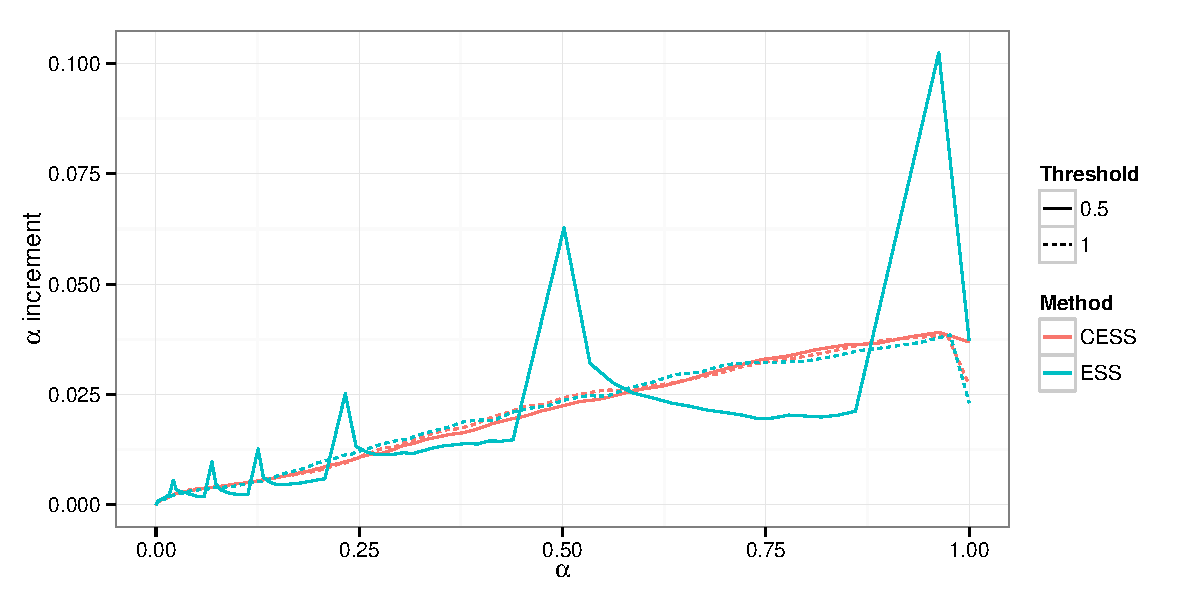
\includegraphics[width=\linewidth]{fig/Adaptive_Dist}
  \caption[Variations of the distribution specification parameter for the
  \protect\pet compartmental model using adaptive \protect\smc algorithms]
  {A typical plot of $\alpha_t - \alpha_{t-1}$ against $\alpha_t$ (for the
    \pet compartmental model using \smc[2] algorithm.) The specifications of
    the adaptive parameter (\ess or \cess) are adjusted such that all four
    samplers use roughly the same number of distributions.}
  \label{fig:adaptive_alpha}
\end{figure}

More specifically, in practice, when using \cess to adaptively place
distributions, a value $\cess^\star \in (0, 1)$ is chosen, and at each
iteration $t$, $\alpha_t$ is chosen such that $\cess_t = \cess^\star$ (with a
preset numeric error tolerance). Figure~\ref{fig:adaptive_alpha} shows the
variation of $\alpha_t$ when fixed reductions in \ess and \cess are used to
specify the sequence of distributions both when resampling is conducted during
every iteration (or equivalently, when the value of $\ess/N$ falls below a
threshold of $1.0$, where $N$ is the number of particles) and when resampling
is conducted only when the value of $\ess/N$ falls below a threshold of $0.5$.
It is found that for the simulated \pet data sets, the \cess-based scheme
leads to a reduction in estimator variance around 20\% relative to a manually
tuned ($\alpha_k(t/T) = (t/T)^5$) schedule while the \ess-based strategy
provides little improvement over the linear case ($\alpha_k(t/T) = t/T$)
unless resampling is conducted during every iteration. The effect for the real
data sets, which vary considerably from each as seen in
Figure~\ref{fig:typical real pet}, is more prominent. The variance reduction
can more than 50\% when using the \cess-based strategy. More performance
comparisons for various settings of the samplers can be found in
Section~\ref{sub:Nonlinear ordinary differential equations}
and~\ref{sub:Positron Emission Tomography compartmental model}.

\subsubsection[cess*, number of distributions, and estimator variance]
{$\cess^\star$, number of distributions, and estimator variance}
\label{ssub:cess*, number of distributions, and estimator variance}

It is intuitively to see that, when using a \cess-based adaptive scheme, where
at each iteration $t$, $\cess_t$ is fixed with a value $\cess^\star$, the more
close $\cess^\star/N$ is to $1$, the larger number of distributions will be placed
and better estimates can be obtained. Unfortunately it is not trivial to
establish a quantitative relations among these three quantities even
asymptotically. However, it is straightforward to conduct an empirical study
of these relations.

We consider the simulated \pet data set using the \smc[2] sampler with 1,000
particles. Figure~\ref{fig:cess iter mean} plots the average number of
distributions (from 100 simulations for each value of $\cess^\star$) against the
value of $(1 - \cess^\star/N)$ on log scales. It can be seen that the number of
distributions is proportional to $(1 - \cess^\star/N)^{-1}$. This relation
holds even for sampler configurations where a very small number of
distributions are used. Similarly, Figure~\ref{fig:cess path var} shows the
relation between the variance of path sampling estimator and the value of
$\cess^\star$. Similar relations can be observed for the standard estimator
(Equation~\eqref{eq:smc2-ds}), which is not shown here.

\begin{figure}[t]
  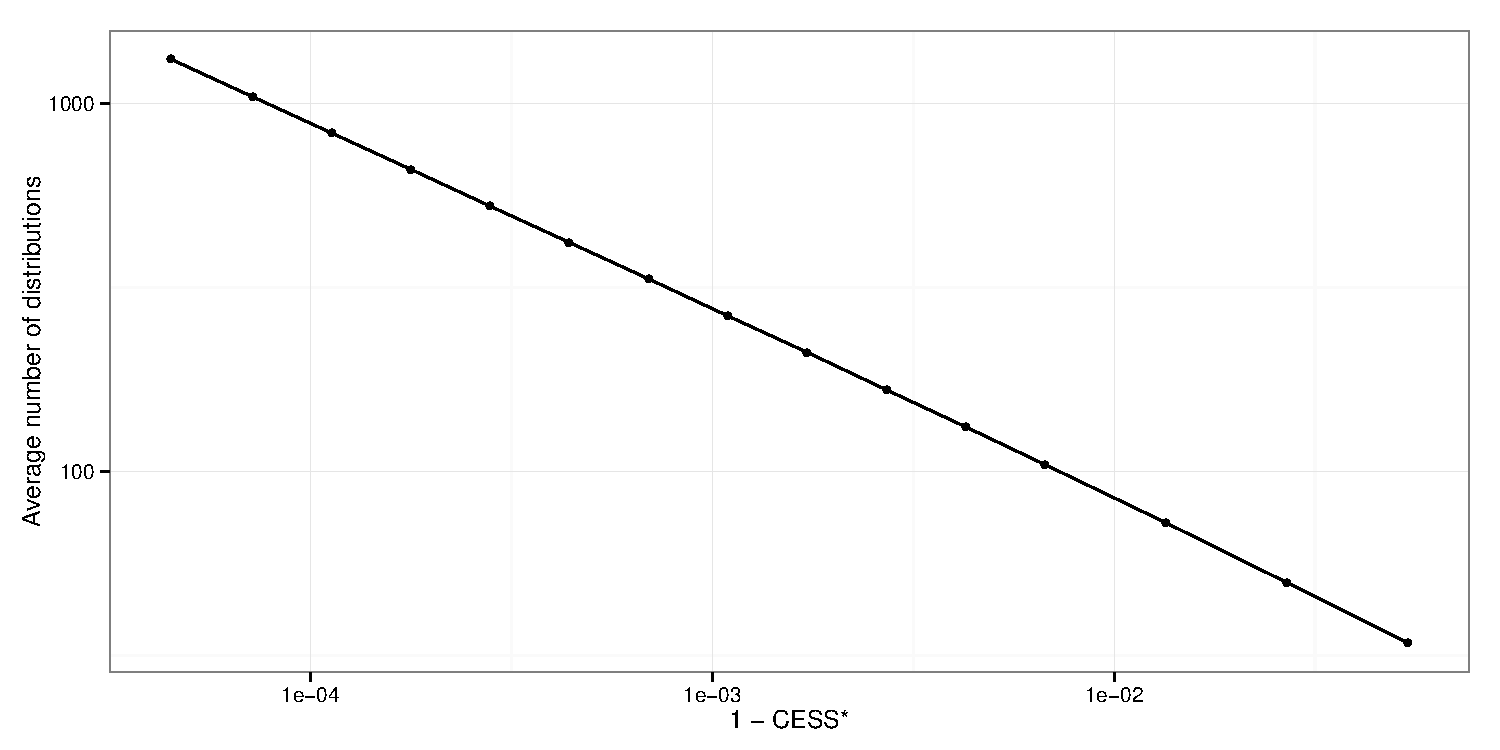
\includegraphics[width=\linewidth]{fig/CESS_Iter_Mean}
  \caption[Relations between average number of distributions and
  \protect\cess]
  {Relations between average number of distributions and
    $\cess^\star$. The number of distributions ranges from $\sim$30 to
    $\sim$1,300.}
  \label{fig:cess iter mean}
\end{figure}

\begin{figure}[t]
  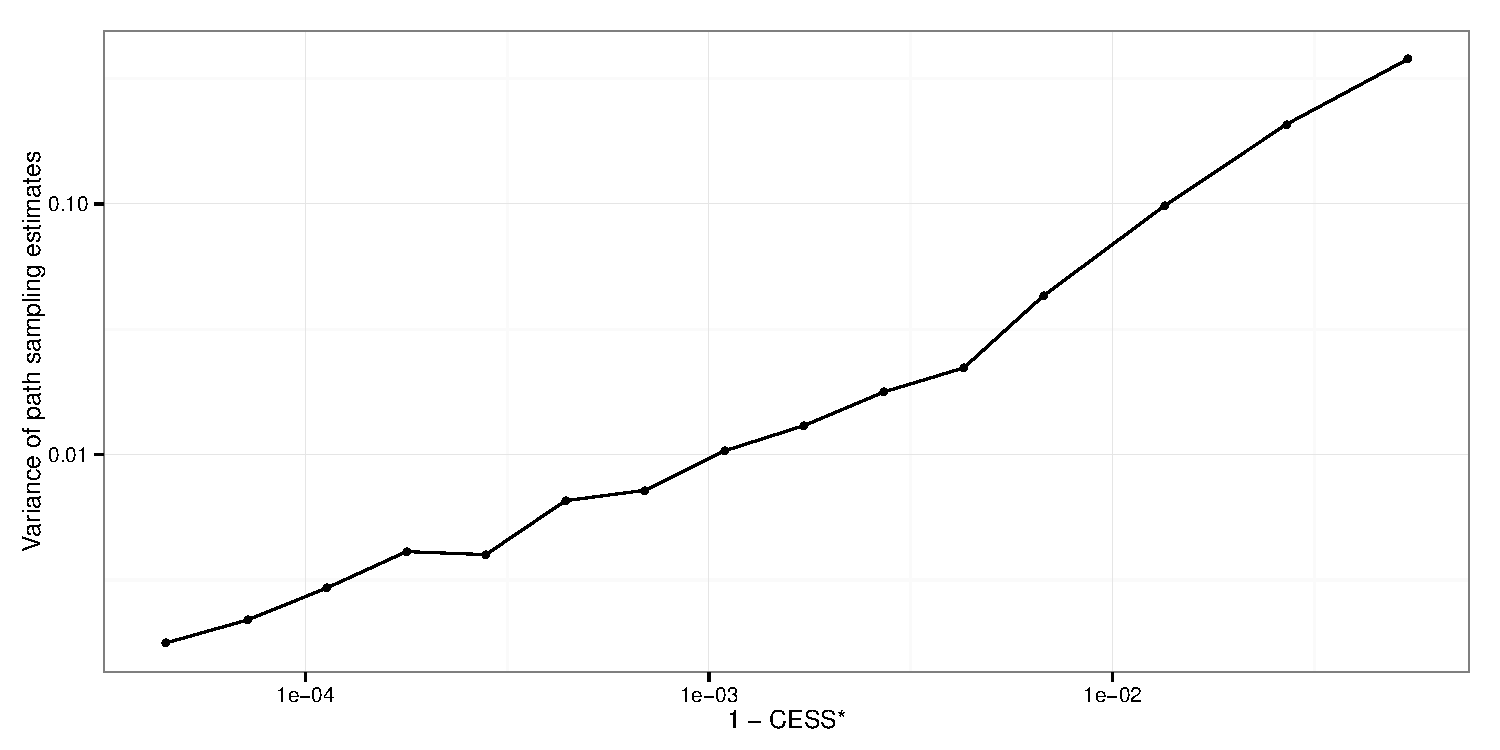
\includegraphics[width=\linewidth]{fig/CESS_Path_Var}
  \caption[Relations between the variance of the path sampling estimator and
  \protect\cess]
  {Relations between the variance of the path sampling estimator and
    $\cess^\star$.}
  \label{fig:cess path var}
\end{figure}

Though the coefficient of the proportionality varies for different
applications or data sets, the relation shown in figures~\ref{fig:cess iter
  mean} and~\ref{fig:cess path var} provide a useful guidelines to select the
value of $\cess^\star$. A small sample experiment can be conducted before using a
value of $\cess^\star$ more close to $1$ to obtain satisfactory estimates or to
utilize given computational resources.

\subsection{Adaptive specification of proposals}
\label{sub:Adaptive specification of proposals}

The \smc sampler is remarkably robust to the mixing speed of the \mcmc kernels
employed as can be seen in the empirical study later. However, as with any
sampling algorithms, faster mixing does not harm performance and in some cases
will considerably improve it. In the particular case of Metropolis-Hastings
kernels, the mixing speed relies on adequate proposal scales.

We use a simpler approach based on \cite{Jasra:2010eh}. They applied an idea
used within adaptive \mcmc methods \cite{Andrieu:2006tw} to \smc samplers by
using variance of parameters estimated from its particle system approximation
as the proposal scales for the next iteration, suitably scaled with reference
to the dimensions of the parameters to be proposed. Although, in practice we
found that such an automatic approach does not always lead to optimal
acceptance rates it generally produces satisfactory results and is simple to
implement. In difficult problems alternative approaches to adaptation could be
employed; one approach demonstrated in \cite{Jasra:2010eh} is to simply employ
a pair of acceptance rate thresholds and to alter the proposal scale from the
simply estimated value whenever the acceptance rate falls outside those
thresholds.

More sophisticated proposal strategies could undoubtedly improve performance
further and warrant further investigation. One possible approach is using the
Metropolis adjusted Langevin algorithm (\mala; see \cite{Roberts:1996vd}.) In
summary, \mala derives a Metropolis-Hastings proposal kernel for a target
$\pi$ which satisfies suitable differentiability and positivity conditions,
from the Langevin diffusion,
\begin{equation*}
  \diff L_t = \frac{1}{2}\nabla\log\pi(L_t)\diff t + \diff B_t
\end{equation*}
where $B_t$ is the standard Brownian motion. Given a state $X^{t-1}$, a new
state is proposed by discrete approximation to the above diffusion. That is,
for a fixed $h>0$,
\begin{equation}
  X^t\sim\calN\Round[bigg]{X^{t-1}+\frac{1}{2}\nabla\log\pi(X^{t-1}), hI_d}
\end{equation}
where $I_d$ is the identity matrix and $d$ is the dimension of the state
space. The new proposed state is accepted or rejected through the usual
Metropolis-Hastings algorithm. Compared to a ``vanilla'' random walk, which
often has very robust theoretical properties, \mala is attractive when it is
possible and its convergence conditions \cite{Roberts:1996vd} can be met,
because only one discrete approximation parameter $h$ needs to be tuned for
optimal performance. In addition, results from \cite{Roberts:2001ta} suggested
that \mala can be more efficient than a random walk when using optimal
scalings. We could also use the particle approximation at time $t - 1$ to
estimate the covariance matrix of $\pi_t$ and thus tune the scale $h$ on-line.
As these algorithms are known to be somewhat sensitive to scaling, and we seek
approaches robust enough to employ with little user intervention, we have not
investigated this strategy here.

\begin{figure}[t]
  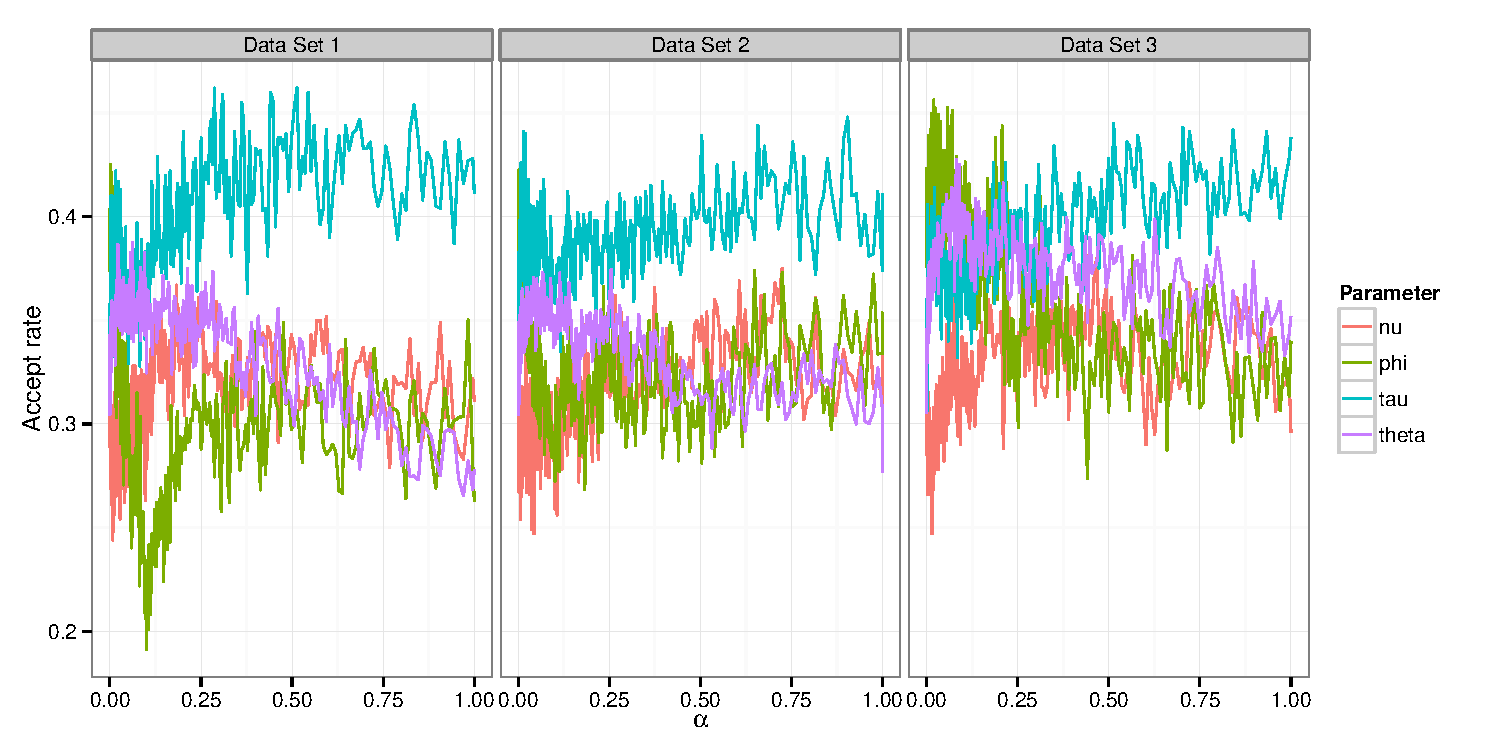
\includegraphics[width=\linewidth]{fig/Adaptive_Proposal}
  \caption[Acceptance rates of adaptive \protect\smc algorithms]
  {Average random walk acceptance rates for \pet compartmental models
    with data sets in Figure~\ref{fig:typical real pet} using adaptive
    proposal scales}
  \label{fig:pet adaptive proposal}
\end{figure}

\begin{figure}[t]
  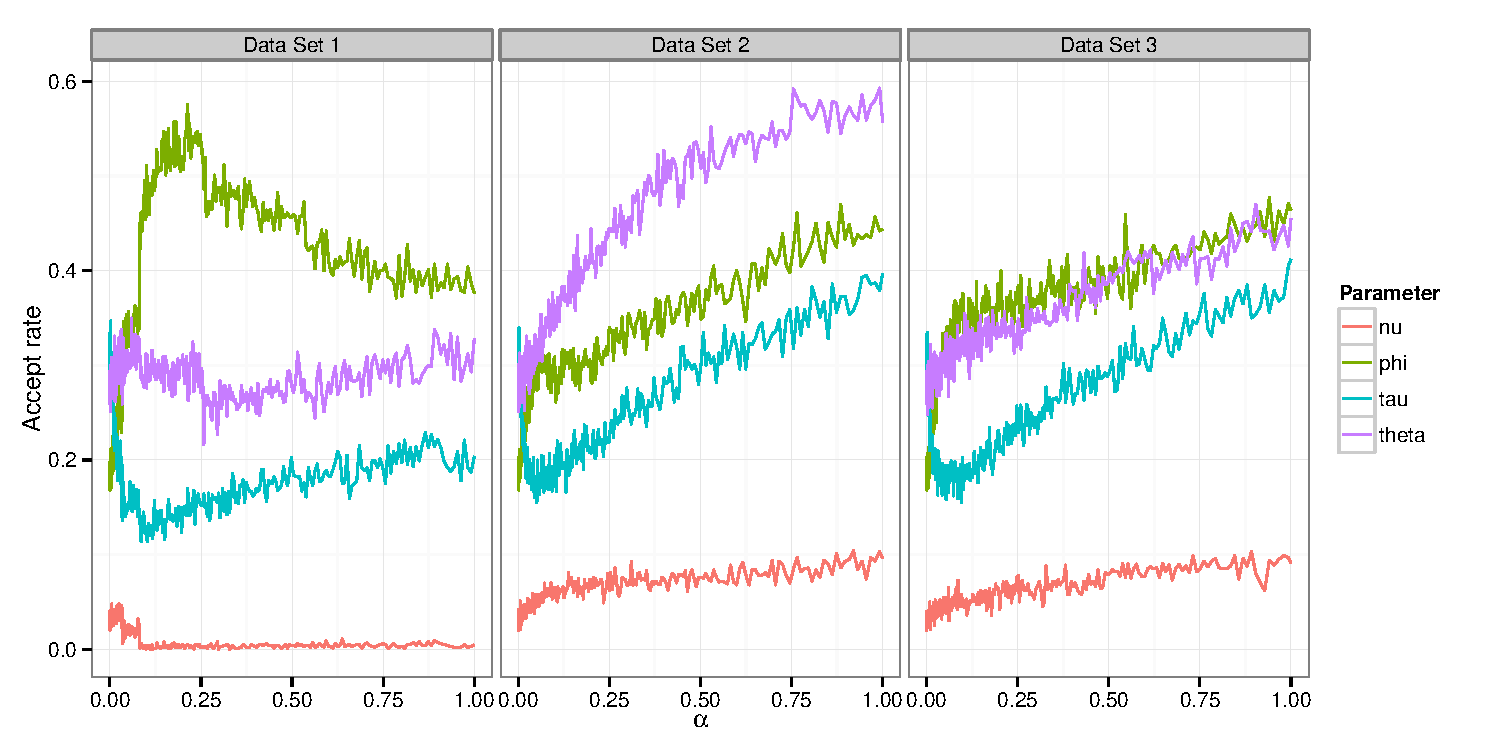
\includegraphics[width=\linewidth]{fig/Fixed_Proposal}
  \caption[Acceptance rates of non-adaptive \protect\smc algorithms]
  {Average random walk acceptance rates for \pet compartmental models
    with data sets in Figure~\ref{fig:typical real pet} using fixed proposal
    scales}
  \label{fig:pet fixed proposal}
\end{figure}

Adaptive specification of proposals is most useful when manual tuning is
difficult or even impossible. We consider the three real \pet data sets shown
in Figure~\ref{fig:typical real pet}. When using adaptive proposal scales, the
average acceptance rates of the four random walk blocks (for parameters
$\phi_{1:r}$, $\theta_{1:r}$, $\tau$ and $\nu$, respectively), is shown in
Figure~\ref{fig:pet adaptive proposal}. Though the results are not close to
the optimal value $0.234$, which is commonly used in practice, they are more
than acceptable. In contrast, in Figure~\ref{fig:pet fixed proposal} we show
the average acceptance rates when using a scheme of proposal scales which is
obtained from another typical real \pet data set. The scheme is tuned such
that for all parameters, the acceptance rates fall within the range $[0.2,
0.4]$ for $\alpha_t \in [0, 1]$. It can be seen that, not only do the results
vary considerably due to the variety of the data sets, which is expected, for
one of the data sets, the parameter $\nu$ fails to move at all. Considering
that there are about a quarter of a million such data sets to be estimated in
a single \pet scan, adaptively specifying the proposal scales is the only
feasible approach. Note that, this problem is not unique to the \pet
compartmental models at all. In many realistic applications, there are a large
number of data sets which vary considerably from each other.

\subsection{An automatic and adaptive algorithm}
\label{sub:An automatic and adaptive algorithm}

With the above refinements, we are ready to implement the \smc[2] algorithm
with minimal tuning and application specific effort while providing robust and
accurate estimates of the model evidence $p(\data|\calM_k)$. First the
geometric annealing scheme that connects the prior $\pi(\theta_k|\calM_k)$ and
the posterior $\pi(\theta_k|\data,\calM_k)$, provides a smooth path for a wide
range of problems.

Second, the actual annealing schedule under this scheme can be determined
through the adaptive schedule as described above. The advantage of the
adaptive schedule will be shown empirically later.

Third, we can adaptively specify the Metropolis random walk (or \mala)
proposal scales through the estimation of their scaling parameters as the
sampler iterates. In contrast to the \mcmc setting, where such adaptive
algorithms will usually require a burn-in period, which will not be used for
further estimation, in \smc, the variance and covariance estimates come at
almost no cost, as all the samples will later be used for marginal likelihood
estimation. Additionally, adaptation within \smc does not require separate
theoretical justification \cite{Beskos:2013vx} -- something which can
significantly complicate the development of effective, theoretically justified
schemes in the \mcmc setting. Alternatively, we can also specify the proposal
scales in a deterministic, but sensible way. Since \smc algorithms are
relatively robust to the change of scales, such deterministic scales will not
require the same degree of tuning as is required to obtain good performance in
\mcmc algorithms.

Though we described the algorithm in the setting of \smc[2], it can also be
applied to other \smc strategies. \smc[1] is less straightforward as the
between model moves still require effort to design and implement. In \smc[3],
the specification of the sequences between posterior distributions are less
generic compared to the geometric annealing scheme in \smc[2]. However, the
adaptive schedule and automatic tuning of \mcmc proposal scales, both can be
applied in these two algorithms in principal. We outline the strategy in
Algorithm~\ref{alg:adaptive}.

\begin{algorithm}
\begin{algorithmic}
  \tophrule
  \STATE \emph{Accuracy control}
  \STATE\STATESKIP Set constant $\cess^\star\in(0,1)$, using a small pilot
  simulation if necessary.

  \STATE \emph{Initialization:} Set $t\leftarrow0$.
  \STATE\STATESKIP Perform the \emph{Initialization} step
    as in Algorithm~\ref{alg:smc1} or~\ref{alg:smc2}

  \STATE \emph{Iteration:} Set $t\leftarrow t + 1$

  \STATE\STATESKIP \emph{Step size selection}
  \STATE\STATESKIP\STATESKIP Use a binary search %(or other search algorithms)
  to find $\alpha^\star$ such that $\cess_{\alpha^\star} = \cess^\star$
  \STATE\STATESKIP\STATESKIP Set $\alpha_t \leftarrow\alpha^\star$ if
    $\alpha^\star \le 1$, otherwise set $\alpha_t\leftarrow1$

  \STATE\STATESKIP \emph{Proposal scale calibration}
  \STATE\STATESKIP\STATESKIP
  Computing the importance sampling estimates of first two moments of
  parameters.
  \STATE\STATESKIP\STATESKIP
  Set the proposal scale of the Markov proposal $K_t$ with the estimated
  parameter variances.

  \STATE\STATESKIP Perform the \emph{Iteration} step as in
  Algorithm~\ref{alg:smc1} or~\ref{alg:smc2} with the found $\alpha_t$
  and proposal scales.

  \STATE \emph{Repeat} the \emph{Iteration} step %up to $t = T$ (or $T_k$ in the
    %case of Algorithm~\ref{alg:smc2})}
    \emph{until $\alpha_t = 1$} then set $T=t$.
  \bottomhrule
\end{algorithmic}
\caption{An Automatic, Generic Algorithm for Bayesian Model Comparison}
\label{alg:adaptive}
\end{algorithm}


As laid out above, the algorithms require minimal tuning. Its robustness,
accuracy and efficiency will be shown in Section~\ref{sec:Performance
  comparison} through comprehensive empirical studies. Here we show some
interesting yet intuitively expected results. We consider the simulated \pet
data sets, using an \smc[2] sampler with 1,000 particles. It is already shown
that using either the adaptive specification of distribution placement or the
\mcmc proposal scales can give better results. The combination of the two can
lead to even better results. The use of the \cess-based schedule scheme will
not only place more distributions where the target distributions changes more
rapidly, but also it will place more distributions where the \mcmc algorithm
mixes slower. To illustrate the idea, we consider four configurations of the
sampler. The proposal scales are specified either adaptively or using a fixed
scheme which is manually tuned. The placement of the distributions is either
\cess-based or using a fixed schedule $\alpha_t = \alpha_k(t/T_k) =
(t/T_k)^5$.

\begin{table}[t]
  \caption[Accuracy of Bayes factor estimates]
  {Bayes factor estimates ($\log B_{1,2}\pm\sd$) for the simulated
    \pet data set using \smc[2] algorithm. All four samplers are configured such
    that about 200 distributions are used.}
  \label{tab:pet four sampler same dist}
  \begin{tabularx}{\linewidth}{lXX}
    \toprule
    & \multicolumn{2}{c}{Proposal scales} \\
    \cmidrule(lr){2-3}
    Schedule & Fixed & Adaptive \\
    \midrule
    Deterministic schedule ($\alpha_k(t/_k) = (t/T_k)^5$) & $1.6\pm0.27$ & $1.6\pm0.22$ \\
    \cess-based adaptive schedule & $1.6\pm0.19$ & $1.6\pm0.15$ \\
    \bottomrule
  \end{tabularx}
\end{table}


The results are shown in Table~\ref{tab:pet four sampler same dist}. More
comprehensive results can be found in Section~\ref{sec:Positron Emission
  Tomography compartmental model}. However, from this particular example, we
can see that the combination of the two adaptive schemes provides superior
performance at very little computation cost. Table~\ref{tab:pet four sampler
  same iter} shows actually equivalent results. Instead of fixing the number
of distributions, we configured the samplers such that they all give roughly
the same precision of the estimates. It is rather obvious to see that the use
of adaptive methods actually give a considerable reduction of computational
cost for a given desired precision of the estimates.

\begin{table}[t]
  \caption[Cost of Bayes factor estimates]
  {Number of distributions used for the simulated \pet data set using
    \smc[2] algorithm. All four samplers are configured such that the Bayes
    factor estimates ($\log B_{1,2}$) have a standard deviation of
    approximately $0.27$.}
  \label{tab:pet four sampler same iter}
  \begin{tabularx}{\linewidth}{lXX}
    \toprule
    & \multicolumn{2}{c}{Proposal scales} \\
    \cmidrule(lr){2-3}
    Schedule & Fixed & Adaptive \\
    \midrule
    Deterministic schedule ($\alpha_k(t/T_k) = (t/T_k)^5$) & $200$ & $182$ \\
    \cess-based adaptive schedule & $175$ & $157$ \\
    \bottomrule
  \end{tabularx}
\end{table}


Although further enhancements and refinements are clearly possible, we focus
in the remainder of this chapter on this simple, generic algorithm which can
be easily implemented in any application and has proved sufficiently powerful
to provide good estimation in the examples we have encountered thus far.

\section{Theoretical considerations}
\label{sec:Theoretical considerations}

The convergence results for the standard estimator can be found in
\cite{DelMoral:2006hc} and references therein. In this work, given our
advocation of \smc[2]-\ps, we extend the results for the path sampling
estimator from \smc samplers. Here we present Proposition~\ref{prop:path_clt},
which is specific to path sampling estimator using the simplest Trapezoidal
approach to numerical integration. It follows as a simple corollary to a more
general result given in Appendix~\appref{sec:Proof of proposition 5.1} which
could be used to characterize more general numerical integration schemes.

\begin{proposition}\label{prop:path_clt}
  Under the same regularity conditions as are required for the central limit
  theorem given in \cite{DelMoral:2006hc} to hold, given an \smc sampler that
  iterates over a sequence of distributions $\{\pi_t =
  \gamma_{\alpha_t}/Z_{\alpha_t}\}_{t=0}^T$ and applies multinomial resampling
  at each iteration, the path sampling estimator, $\hat\Xi_{T}^{N}$, as
  defined in Equation~\eqref{eq:path_est} obeys a central limit theorem in the
  following sense: Let $\xi_t(\cdot) = \frac{\diff\log
    \gamma_{\alpha}(\cdot)}{\diff\alpha}\Bigm|_{\alpha = \alpha_t}$,
  $\beta_{0} = \alpha_0 / 2$, $\beta_{T} = \alpha_T / 2$ and for $t =
  1,\ldots,T-1$, $\beta_t = (\alpha_{t + 1} - \alpha_{t-1})/2$, then,
  provided $\xi_t$ is bounded,
  \begin{equation}
    \lim_{N\to\infty}\sqrt{N}(\hat\Xi_{T}^{N} - \Xi_T)
    \xrightarrow{D}\calN(0, V_T(\xi_{0:T}))
  \end{equation}
  where $V_t$, $0\le t \le T$ is defined by the following recursion,
  \begin{align}
    V_0(\xi_0) =&  \beta_0^2
    \int \pi_0(x_0) (\xi_0(x_0)
    - \pi_0(\xi_0))^2 dx_0 \\
    V_t(\xi_{0:t}) =& V_{t-1}\Round[bigg]{\xi_{0:t-2}, \xi_{t-1}
    + \frac{\beta_t}{\beta_{t-1}}
    \frac{\pi_{t}(\cdot)}{\pi_{t-1}(\cdot)}
    \int K_t(\cdot,x_t) (\xi_t(x_t)-\pi_t(\xi_t)) \intd x_t
    } \\\notag
    &+ \beta_t^2 \int\frac{\pi_t(x_{t-1})^2}{\pi_{t-1}(x_{t-1})}
    K_t(x_{t-1},x_t)(\xi_t(x_t) - \pi_t(\xi_t))^2) \intd x_{t-1} \intd x_t.
  \end{align}
\end{proposition}

Application of similar arguments to those used in \cite{DelMoral:2006hc} to
the historical process associated with the \smc sampler would lead to
essentially the same result, but we find this approach more transparent. We
note that much recent analysis of \smc algorithms has focused on relaxing the
relatively strong assumptions used in the results upon which this result is
based -- looking at more general resampling schemes \cite{DelMoral:2012jq} and
relaxing compactness assumptions \cite{Whiteley:2013vx} for example. However,
we feel that this simple result is sufficient to show the relationship between
the path sampling and simple estimators and that in this instance the
relatively simplicity of the resulting expression justifies these stronger
assumptions.

\section{Performance comparison}
\label{sec:Performance comparison}

In this section, we will use three examples to illustrate the algorithms. The
Gaussian mixture model is discussed first, with implementations for all three
\smc algorithms with comparison to \rjmcmc and population \mcmc. It will be
shown that all five algorithms agree on the results while the performance in
terms of Monte Carlo variance varies considerably. It will also be
demonstrated how the adaptive refinements of the algorithms behaves in
practice. We will reach the conclusion that considering ease of
implementation, performance and generality, the \smc[2] algorithm is most
promising among all three strategies.

Then two more realistic examples, a nonlinear \ode model and the \pet
compartmental model are used to study the performance and robustness of
algorithm \smc[2] compared to \ais and population \mcmc. Various
configurations of the algorithms are considered including both sequential and
parallelized implementations.

The \cpp implementations, which make use of the \vsmc library of
\cite{vsmcjss}, of all examples can be found at
\url{https://github.com/zhouyan/vSMCExample} and the library is also
introduced in Chapter~\ref{cha:vSMC: A C++ Library for Parallel SMC}.

\subsection{Gaussian mixture model}
\label{sub:Gaussian mixture model}

Since \cite{Richardson:1997ea}, the Gaussian mixture model (\gmm) has
provided a canonical example of a model-order-determination problem. We use
the model formulation of \cite{DelMoral:2006hc} to illustrate the efficiency
and robustness of the methods proposed in this paper compared to other
approaches. The model is as follows; data $\data = (y_1,\dots,y_n)$ are
independently and identically distributed as
\begin{equation*}
  y_i|\theta_r \sim \sum_{j=1}^r \omega_j\calN(\mu_j,\lambda_j^{-1})
\end{equation*}
where $\calN(\mu_j,\lambda_j^{-1})$ denotes the Normal distribution with mean
$\mu_j$ and precision $\lambda_j$; $\theta_r =
(\mu_{1:r},\lambda_{1:r},\omega_{1:r})$ and $r$ is the number of components in
each model. The parameter space is thus $\Real^r \times (\Real^{+})^r\times
\Delta_r$ where $\Delta_r = \{\omega_{1:r}:0\le\omega_j\le1;
\sum_{j=1}^r\omega_j=1\}$ is the standard $r$-simplex. The priors which are
the same for each component are taken to be $\mu_j\sim\calN(\xi,\kappa^{-1})$,
$\lambda_j\sim\calGa(\nu,\chi)$ and $\omega_{1:r}\sim\calD(\rho)$ where
$\calD(\rho)$ is the symmetric Dirichlet distribution with parameter $\rho$
and $\calGa(\nu,\chi)$ is the Gamma distribution with shape $\nu$ and scale
$\chi$. The prior parameters are set in the same manner as in
\cite{Richardson:1997ea}. Specifically, let $y_{\text{\textsc{min}}}$ and
$y_{\text{\textsc{max}}}$ be the minimum and maximum of data $\data$, the
prior parameters are set such that
\begin{equation*}
  \xi = (y_{\text{\textsc{max}}} + y_{\text{\textsc{min}}}) / 2, \quad
  \kappa = (y_{\text{\textsc{max}}} - y_{\text{\textsc{min}}})^{-2}, \quad
  \nu = 2, \quad \chi = 50\kappa, \quad \rho = 1
\end{equation*}
The data is simulated from a four components model with $\mu_{1:4} = (-3, 0,3,
6)$, and $\lambda_j =2$, $\omega_j = 0.25$, $j = 1,\dots,4$.

We consider several algorithms. First the \rjmcmc algorithm as in
\cite{Richardson:1997ea}, and second an implementation of the \smc[1]
algorithm. Next \ais, population \mcmc and \smc[2] are used for within-model
simulations. The last is an implementation of the \smc[3] algorithm. In all
the algorithms, the local move which does not change the dimension of the
model is constructed as a composition of Metropolis-Hastings random walk
kernels:
\begin{enumerate}
  \item Update $\mu_{1:r}$ using a multivariate Normal random walk proposal.
  \item Update $\lambda_{1:r}$ using a multivariate Normal random walk on
    logarithmic scale, i.e., on $\log\lambda_{j}$, $j = 1, \dots, r$.
  \item Update $\omega_{1:r}$ using a multivariate Normal random walk on logit
    scale, i.e., on $\omega_{j}/\omega_r$, $j = 1,\dots,r-1$.
\end{enumerate}
The \rjmcmc, \smc[1] and \smc[3] algorithms use two additional
reversible jump moves. The first is a combine and split move; the second is a
birth and death move. Both are constructed in the same manner as in
\cite{Richardson:1997ea}. Also in these implementations, an adjacency
condition was imposed on the means $\mu_{1:r}$, such that $\mu_1 < \mu_2 <
\dots < \mu_r$. No such restriction was used for other algorithms.

In the \smc[1], \smc[2], \ais and the population \mcmc implementations, the
distributions are chosen with a geometric schedule, i.e., as in
Equation~\eqref{eq:geometry_1} for \smc[1] and Equation~\eqref{eq:geometry_2}
for the other three. This annealing scheme has been used in
\cite{DelMoral:2006hc,Jasra:2007in} and many other works. The geometric scheme
can also be seen in \cite{Calderhead:2009bd} for population \mcmc tempering. A
schedule $\alpha(t/T) = (t/T)^p$, with $p = 2$ was used. The rationale behind
this particular schedule can be seen in \cite{Calderhead:2009bd} and other
values of $p$ were also tried while $p\approx2$ performs best in this
particular example. The adaptive schedule was also implemented for \smc[2] and
\ais algorithms.

The proposal scales for each block of the random walks are specified
dynamically according to values of $\alpha(t/T)$ for the \smc[2] and \ais
algorithms and also manually tuned for other algorithms such that the
acceptance rates fall in $[0.2, 0.5]$. Later for the \smc[2] and \ais
algorithms, we also consider adaptive schedule of the distribution
specification parameter $\alpha(t/T)$ and the proposal scales of the random
walks.

For \smc[2], \smc[3] and \ais we consider both the direct estimator and the
path sampling estimator. For population \mcmc we consider the path sampling
estimator.

\subsubsection{Results}
\label{sec:gmm_res}

The \smc[1] implementation uses 10,000 particles and 500 distributions. The
\rjmcmc implementation uses five million iterations in addition to one million
iterations of burn-in period. The resulting estimates of model probabilities
are shown in Table~\ref{tab:gmm-prob}.

The \smc[2], \smc[3] and \ais implementations use 1,000 particles and 500
iterations. The population \mcmc implementation uses 50 chains and 10,000
iterations in addition to 10,000 iterations of burn-in period -- these
implementations have approximately equal computational costs. From the results
obtained under the \smc[1] and \rjmcmc algorithms it is clear that, in this
particular example, simulations for models with fewer than ten components are
adequate to characterize the model space. Therefore, under this configuration,
the cost is roughly the same in terms of computational resources as that of
the \smc[1] and \rjmcmc algorithms. From the results of \rjmcmc and \smc[1],
we consider the four and five components models (i.e., the true model and the
most competitive one amongst the others). The estimates are shown in
Table~\ref{tab:gmm-pair} which, like all of the other tables in this section,
summarizes the Monte Carlo variability of 100 replicate runs of each
algorithm.

\draftnote{There are still some overfull boxes in this
  Table~5.3, but it shall look just fine once I drop the
  draft option of the document class and do not show the overfull bars}

\begin{table}[t]
  \linespread{1.1}\selectfont
  \caption
  [Gaussian mixture model posterior model probability]
  {Gaussian mixture model posterior model probability estimates obtained via
    \smc[1] and \rjmcmc.}
  \label{tab:gmm-prob}
  \begin{tabu}{X[2l]X[2.5l]X[1c]X[1c]X[1c]X[1c]X[1l]X[1c]X[1c]}
    \toprule
    & & \multicolumn{7}{c}{Number of components} \\
    \cmidrule(lr){3-9}
    Quantity & Algorithm & $\le2$ & $3$ & $4$ & $5$ & $6$ & $7$ & $\ge8$ \\
    \midrule
    $\Prob(\calM_k|\data)$ & \smc[1]
    & $0$ & $0.0022$ & $0.89$ & $0.10$ & $0.0064$ & $0.0014$ & $0$ \\
    & \rjmcmc
    & $0$ & $0.0013$ & $0.89$ & $0.10$ & $0.0062$ & $0.0025$ & $0$ \\
    $\log B_{4,k}$     & \smc[1]
    & $\infty$ & $6.00$ & $0$ & $2.15$ & $4.93$ & $6.45$ & $\infty$ \\
    & \rjmcmc
    & $\infty$ & $6.53$ & $0$ & $2.15$ & $4.97$ & $5.87$ & $\infty$ \\
    \bottomrule
  \end{tabu}
\end{table}

\begin{table}
  \begingroup\small\begin{tabularx}{\linewidth}{lRRRRRRR}
    \toprule
    & \multicolumn{7}{c}{Algorithms} \\
    \cmidrule(lr){2-8}
    Quantity
    & \smc[2]-\ds & \smc[2]-\ps & \smc[3]-\ds & \smc[3]-\ps & \ais-\ds & \ais-\ps &
    \pmcmc \\
    \midrule
    $\log B_{4,5}$
    & $2.15$ & $2.15$ & $2.16$ & $2.21$ & $2.16$ & $2.17$ & $2.63$ \\
    \sd
    & $0.25$ & $\color{MRed}{0.22}$
    & $0.61$ & $0.62$ & $1.12$ & $1.10$ & $0.41$ \\
    \bottomrule
  \end{tabularx}\endgroup
  \caption{Gaussian mixture model estimates obtained via \smc[2], \smc[3], \ais
    and \pmcmc}
  \label{tab:gmm-pair}
\end{table}


From Tables~\ref{tab:gmm-prob} and~\ref{tab:gmm-pair}, it can be seen that the
standard estimators (\rjmcmc, \smc[1], \smc[2]-\ds, \smc[3]-\ds and \ais-\ds)
agree with each other. Among the path sampling estimators, \smc[2]-\ps and
\ais-\ps have little bias. \smc[3]-\ps shows a little more bias. The
population \mcmc algorithm has a considerably larger bias as the number of
distributions is relatively small (as noted previously, a larger number will
negatively affect the mixing speed). In terms of Monte Carlo variance, in
Table~\ref{tab:gmm-pair}, \smc[2] clearly has an advantage compared to its
no-resampling variant, \ais. The differences of Monte Carlo standard deviation
between \smc[2], \smc[3] and the population \mcmc, although they do not affect
model selection in this particular example, are considerable.

\paragraph{Effects of resampling}

It is clear from these results that resampling (when required) can
substantially improve the estimation of normalizing constants within an \smc
framework. This does not contradict the statement in \cite{DelMoral:2006hc}
which suggests that resampling may not much help when the normalizing constant
is the object of interest, the theoretical argument which supports this relies
upon the assumption that the Markov kernel used to mutate the particles mixes
extremely rapidly and the result is obtained under the assumption that
resampling is performed after every iteration. When the Markov kernel is not
so rapidly mixing, the additional stability provided by the resampling
operation can outweight the attendant increase in Monte Carlo variance and
that is what we observed here (and in the case of the other examples
considered below; results not shown.)

\begin{figure}
  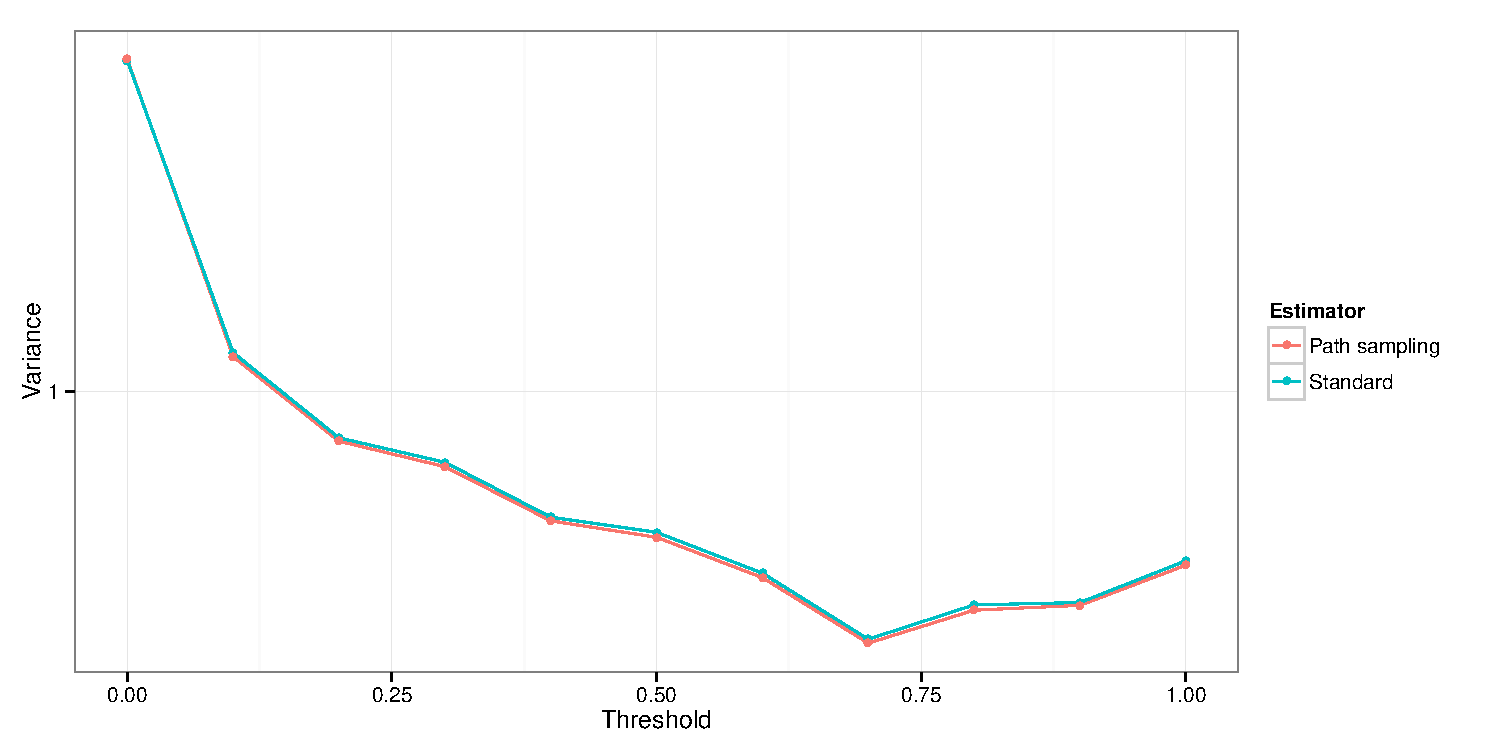
\includegraphics[width=\linewidth]{fig/GMM_Resample}
  \caption[Variance of standard standard estimator and path sampling using
  adaptive resampling]
  {Monte Carlo variance of standard estimator and path sampling
    estimator using different threshold of $\ess/N$ for Gaussian mixture model
    with \smc[2] algorithm. The variances are plotted on log scale}
  \label{fig:gmm resample}
\end{figure}

On the other hand, in this work we advocate resampling adaptively instead of
resampling every iteration. The proposed adaptive schedule also has
significant advantage in this situation. It is of interest to see if adaptive
resampling has performance improvement when compared to resampling every
iteration. We consider using the \smc[2] algorithm with 1,000 particles, 100
distributions scheduled as $\alpha(t/T) = (t/T)^2$, and various threshold of
$\ess/N$ under which resampling is performed. The Monte Carlo variance of both
the standard estimator and the path sampling estimator is shown in
Figure~\ref{fig:gmm resample}. It can be shown that neither performing
resampling every iteration or never performing resampling (i.e., the \ais
algorithm), gives optimal results. Though it may be difficult to determine an
optimal value, the commonly used value $0.5$ seems to be suitable for this
particular example, in the sense that the variance is only slightly higher
than that of an sampler performing resampling at every iteration while the
computational cost is reduced. The reduction in computational cost might be
negligible for some applications. However, as noted before, when parallel
computing is considered, frequent resampling can be a bottleneck of
performance in reality.

\paragraph{Effects of adaptive schedules}

To assess the evolution of distributions with an adaptive schedule, we
consider the relation between $\alpha_t - \alpha_{t-1}$ and $\alpha_t$. As
stated before, one of the motivations of using \cess for adaptive placement of
distribution is to ensure that $\alpha_t$ evolves the same path regardless the
resampling strategies. Earlier in Figure~\ref{fig:adaptive_alpha} we showed
the evolution of $\alpha_t$ when fixing \ess or \cess and resampling every
iteration or only when $\ess/N < N$, where $N$ is the number of particles. As
shown in the plot, when fixing \cess, the evolution of the distributions is
not affected by the resampling strategy.  In contrast, fixing \ess yields a
sequence of distributions which depends strongly upon the resampling strategy.

In terms of the actual performance when using the \cess adaptive strategy in
the \smc[2] and \ais algorithms, a reduction of standard deviation of 20\% was
observed comparing to $\alpha(t/T) = (t/T)^2$, the one shown in
Table~\ref{tab:gmm-pair}. When applied to the \smc[3] algorithm, 50\%
reduction was observed. If the \ess adaptive strategy is used instead, similar
standard deviation reduction is observed when resampling is performed every
iteration but no significant effect was observed when resampling was only
performed when $\ess/N < 0.5$ (i.e., using \ess rather than \cess entirely
eliminated the benefit.)

\paragraph{Effects of adaptive proposal scales}

When using the \smc[2] algorithm, if the adaptive strategy of
\cite{Andrieu:2006tw} is applied, where the important sampling estimates of
the variance of parameters are included in the adaptation, the acceptance
rates fall within $[0.2, 0.5]$ dynamically without manual tuning as for the
results in Table~\ref{tab:gmm-pair}. It should be noted that in this
particular example, it is the variance of $\log\lambda_{1:r}$ being estimated
as the corresponding random walk block operates on the log scale. The same
principle applies to the weight parameters $\omega_{1:r}$, which have random
walks on the logit scale. Approximately 20\% reduction in standard deviation
was observed.

\subsection{Nonlinear ordinary differential equations}
\label{sub:Nonlinear ordinary differential equations}

The example from the previous section suggests that \smc[2] performs well
relative to the other \smc possibilities. Given the wide range of settings in
which it can be easily deployed, we will now concentrate further on this
method. It also suggests that in the simple case of Gaussian mixtures, a
complete adaptive strategy for both distribution specification and proposal
scales works well. In this section, this will now be further explored in a
more complex model, a nonlinear ordinary differential equations (\ode) system.
This model, which was studied in \cite{Calderhead:2009bd}, is known as the
Goodwin model. The \ode system, for an $m$-component model, is:
\begin{align*}
  \frac{\diff X_1(t)}{\diff t} &= \frac{a_1}{1 + a_2 X_m(t)^{\rho}}
  - \alpha X_1(t)  & \\
  \frac{\diff X_i(t)}{\diff t} &= k_{i-1}X_{i-1}(t) - \alpha X_i(t)
  & i = 2,\dots,m \\
  X_i(0) &= 0 & i = 1,\dots,m
\end{align*}
The parameters $\{\alpha,a_1,a_2,k_{1:m-1}\}$ have common prior distribution
$\calGa(0.1, 0.1)$. Under this setting, $X_{1:m}(t)$ can exhibit either
unstable oscillation or a constant steady state. The data are simulated for
$m=\{3,5\}$ at equally spaced time points from $0$ to $60$, with time step
$0.5$. The last 80 data points of $(X_1(t), X_2(t))$ are used for inference.
Normally-distributed noise with standard  deviation $\sigma=0.2$ is added to
the simulated data. Following \cite{Calderhead:2009bd}, the variance of the
additive measurement error is assumed to be known. Therefore, the posterior
distribution has $m+2$ parameters for an $m$-component model.

As shown in \cite{Calderhead:2009bd}, when $\rho > 8$, due to the possible
instability of the \ode system, the posterior can have a considerable number
of local modes. In this example, we set $\rho = 10$. Also, as the solution to
the \ode system is somewhat unstable, slightly different data can result in
very different posterior distributions.

\subsubsection{Results}

We compare results from the \smc[2] and population \mcmc algorithms. For the
\smc implementation, 1,000 particles and 500 iterations were used, with the
distributions specified specified by Equation~\eqref{eq:geometry_2}, with
$\alpha_k(t/T_k) = (t/T)^5$, or via the completely adaptive specification. For
the population \mcmc algorithm, 50,000 iterations are performed for the
adaptation of the proposal scales (the burn-in period), and another 10,000
iterations are used for inference. The same tempering as was used for \smc is
used here. Note that, in a sequential implementation of population \mcmc, with
each iteration updating one local chain and attempting a global exchange, the
computational cost of after burn-in iterations is roughly the same as the
entire \smc algorithm. In addition, changing $T$ within the range of the
number of cores available does not substantially change the computational cost
of a generic parallel implementation of the population \mcmc algorithm. We
compare results from $T = 10,30,$ and~$100$.

The results for data generated from the simple model ($m = 3$) and complex
model ($m = 5$), again summarizing variability amongst 100 runs of each
algorithm, are shown in Table~\ref{tab:node-s} and~\ref{tab:node-c},
respectively.

\newgeometry{hmargin={1in,1in},vmargin={1in,2in},bindingoffset=\mclassbinding}

\begin{table}
  \UseAltLinespread
  \caption
  [Nonlinear \protect\ode model marginal likelihood and the Bayes factor
  estimates (simple model data)]
  {Nonlinear \ode model marginal likelihood and the Bayes factor estimates
    with data generated from a simple (three components) model.}
  \label{tab:node-s}
  \begin{tabu}{X[0.3l]X[0.8c]X[0.8c]X[0.8c]X[1r]X[1r]X[1r]}
    \toprule
    &&&& \multicolumn{2}{c}{Marginal likelihood} & Bayes factor \\
    &&&& \multicolumn{2}{c}{$\log p(\data|\calM_k)\pm\sd$} & $\log B_{3,5}\pm\sd$ \\
    \cmidrule(lr){5-6}
    $T$   & Proposal & Annealing & Algorithm   & $r = 3$                & $r = 5$                & \\ \midrule
    $10 $ & Manual         & Prior (5) & \pmcmc      & $-109.7\pm3.2$         & $-120.3\pm2.5$         & $10.6\pm3.8$ \\
    $30 $ &                &           &             & $\SubBest{-105.0\pm1.2}$ & $\SubBest{-116.1\pm2.2}$ & $\SubBest{11.2\pm2.5}$ \\
    $100$ &                &           &             & $-134.7\pm7.9$         & $-144.1\pm6.2$         & $9.4\pm11.2$ \\ \midrule
    $500$ & Manual         & Prior (5) & \smc[2]-\ds & $-104.6\pm2.0$         & $-112.7\pm1.8$         & $8.1\pm2.8$ \\
          &                &           & \smc[2]-\ps & $-104.5\pm1.8$         & $-112.7\pm1.5$         & $8.2\pm2.5$ \\
    $500$ & Manual         & Adaptive  & \smc[2]-\ds & $-104.5\pm1.1$         & $-112.7\pm1.1$         & $8.1\pm1.6$ \\
          &                &           & \smc[2]-\ps & $-104.6\pm1.0$         & $-112.8\pm1.0$         & $8.2\pm1.5$ \\
    $500$ & Adaptive       & Adaptive  & \smc[2]-\ds & $-104.5\pm0.5$         & $-112.7\pm0.4$         & $8.1\pm0.8$ \\
          &                &           & \smc[2]-\ps & $\Best{-104.6\pm0.4}$    & $\Best{-112.8\pm0.3}$    & $\Best{8.1\pm0.6}$ \\
    \bottomrule
    \multicolumn{7}{r}{%
      \begin{minipage}{\linewidth-2em}\vskip1ex\sffamily
        $T$: The number of distributions.

        Proposal: The proposal scales of the \mcmc kernels.

        Annealing: The annealing scheme of the distributions,
        $\alpha_k(t/T_k)$ in Equation~\ref{eq:geometry_2}.

        \Best: The estimate with the smallest variance among all algorithms
        settings.

        \SubBest: The estimate with the smallest variance for a single
        algorithm (\smc[2] or \pmcmc) among different settings.
      \end{minipage}}
  \end{tabu}
\end{table}

\begin{table}
  \UseAltLinespread
  \caption
  [Model selection results of nonlinear \protect\ode model using the Bayes factor (simple model data)]
  {Frequencies of models selected by the Bayes factor (\%) for the nonlinear \ode model with data generated from a simple (three components) model.}
  \label{tab:node-s-mo}
  \begin{tabu}{X[0.3l]X[0.8c]X[0.8c]X[0.8c]X[0.2r]X[0.2r]X[0.2r]X[0.2r]X[0.2r]}
    \toprule
    &&&& \multicolumn{5}{c}{Number of components}\\
    \cmidrule(lr){5-9}
    $T$   & Proposal       & Annealing & Algorithm   & $2$ & $  3$ & $4$ & $5$ & $6$ \\ \midrule
    $10 $ & Manual         & Prior (5) & \pmcmc      & $2$ & $ 96$ & $2$ & $0$ & $0$ \\
    $30 $ &                &           &             & $0$ & $100$ & $0$ & $0$ & $0$ \\
    $100$ &                &           &             & $0$ & $100$ & $0$ & $0$ & $0$ \\
    $500$ & Manual         & Prior (5) & \smc[2]-\ds & $0$ & $100$ & $0$ & $0$ & $0$ \\
          &                &           & \smc[2]-\ps & $0$ & $100$ & $0$ & $0$ & $0$ \\
    $500$ & Manual         & Adaptive  & \smc[2]-\ds & $0$ & $100$ & $0$ & $0$ & $0$ \\
          &                &           & \smc[2]-\ps & $0$ & $100$ & $0$ & $0$ & $0$ \\
    $500$ & Adaptive       & Adaptive  & \smc[2]-\ds & $0$ & $100$ & $0$ & $0$ & $0$ \\
          &                &           & \smc[2]-\ps & $0$ & $100$ & $0$ & $0$ & $0$ \\
    \bottomrule
    \multicolumn{9}{r}{%
      \begin{minipage}{\linewidth-2em}\vskip1ex\sffamily
        $T$: The number of distributions.

        Proposal: The proposal scales of the \mcmc kernels.

        Annealing: The annealing scheme of the distributions,
        $\alpha_k(t/T_k)$ in Equation~\ref{eq:geometry_2}.
      \end{minipage}}
  \end{tabu}
\end{table}

%\restoregeometry

\begin{table}
  \caption{Nonlinear \ode model marginal likelihood and Bayes factor estimates
    with data generated from simple (three components) model.}
  \label{tab:node-c}
  \begin{tabu}{X[1l]X[2c]X[2c]X[2c]X[4r]X[4r]X[6r]}
    \toprule
    &&&& \multicolumn{2}{c}{Marginal likelihood ($\log p(\data|\calM_k)\pm\sd$)} & Bayes factor ($\log B_{3,5}\pm\sd$) \\
    \cmidrule(lr){5-6}
    $T$   & Proposal & Annealing & Algorithm   & $m = 3$                 & $m = 5$                & \\ \midrule
    $10 $ & Manual   & Prior (5) & \pmcmc      & $-1651.0\pm27.9$        & $-85.1\pm36.6$         & $1565.9\pm42.1$ \\
    $30 $ &          &           &             & $\SubBest-1639.7\pm7.4$ & $\SubBest-78.9\pm11.2$ & $\SubBest1560.8\pm12.8$ \\
    $100$ &          &           &             & $-1624.6\pm15.7$        & $-75.7\pm24.8$         & $1548.9\pm25.6$ \\ \midrule
    $500$ & Manual   & Prior (5) & \smc[2]-\ds & $-1640.7\pm10.8$        & $-78.5\pm9.8$          & $1562.2\pm10.1$ \\
          &          &           & \smc[2]-\ps & $-1640.8\pm 8.4$        & $-79.2\pm7.9$          & $1561.6\pm 8.5$ \\
    $500$ & Manual   & Adaptive  & \smc[2]-\ds & $-1639.7\pm 6.9$        & $-78.6\pm4.8$          & $1561.1\pm7.1$ \\
          &          &           & \smc[2]-\ps & $-1640.1\pm 5.4$        & $-78.8\pm3.7$          & $1561.3\pm6.8$ \\
    $500$ & Adaptive & Adaptive  & \smc[2]-\ds & $-1639.8\pm 2.2$        & $-79.4\pm1.7$          & $1560.4\pm3.1$ \\
          &          &           & \smc[2]-\ps & $\Best-1640.2\pm 1.9$   & $\Best-78.5\pm1.5$     & $\Best1561.7\pm2.3$ \\
    \bottomrule
    \multicolumn{7}{r}{%
      \begin{minipage}{\linewidth-2em}\vskip1ex\sffamily
        $T$: The number of distributions. That is, the number parallel \mcmc
        chains for \pmcmc algorithm and the number of iterations for the \smc
        algorithm. For the \pmcmc algorithm, at each iteration, a single \mcmc
        chain is chosen randomly to be updated. There is a 50,000 iterations
        burin period and another 10,000 iterations are used for inference. For
        the \smc algorithm, 1,000 particles are used.

        Proposal: The proposal scales of the \mcmc kernels. The ``Manual''
        proposal is manually tuned such that the accept rates fall between
        $[0.2, 0.6]$. The ``Adaptive'' proposal is dynamically set using
        moments estimates from the last iteration of the particle system.

        Annealing: The annealing scheme of the distributions, $\alpha(t/T_k)$
        in Equation~\ref{eq:geometry_2}. The ``Prior (5)'' scheme is
        concentrated around the prior distribuiton, with $\alpha(t/T_k) =
        (t/T_k)^5$. The ``Adaptive'' scheme set $\alpha$ dynamically such that
        for each iteration, \cess is a constant. The constant value of \cess
        is chosen such that on average, 500 iterations was produced.

        \Best: The estimate with the smallest variance among all algorithms
        settings.

        \SubBest: The estimate with the smallest variance for a single
        algorithm (\smc[2] or \pmcmc) among different settings.
      \end{minipage}}
  \end{tabu}
\end{table}


As shown in both cases, the number of distributions can affect the performance
of population \mcmc algorithms considerably. When using 10 distributions,
large bias from numerical integration for path sampling estimator was
observed, as expected. With 30 distributions, the performance is comparable to
the \smc[2] sampler, though some bias is still observable. With 100
distributions, there is a much larger variance because, with more chains, the
information travels more slowly from rapidly mixing chains to slowly mixing
ones and consequently the mixing of the overall system is inhibited.

The \smc algorithm provides results comparable to the best of
three population \mcmc implementations in essentially all settings, including
one in which both the annealing schedule and proposal scaling were fully
automatic. In fact, the completely adaptive strategy was the most successful.

It can be seen that increasing the number of distributions not only reduces
the bias of numerical integration for path sampling estimator, but also
reduces the variance considerably. On the other hand increasing the number of
particles can only reduce the variance of the estimates, in accordance with
the Central Limit Theorem (see \cite{DelMoral:2006hc} for the standard
estimator and extensions for path sampling estimator,
Proposition~\ref{prop:path_clt}). The bias arises from the numerical
integration scheme and cannot be reduced by using more particles. Though there
exists the trade-off between the number of particles and the number
distributions, increasing either of them can always benefit the accuracy of
the estimators. We will study this trade-off more carefully with the next more
realistic example.

\subsection{Positron Emission Tomography compartmental model}
\label{sub:Positron Emission Tomography compartmental model}

It is now interesting to compare the proposed algorithm with other
state-of-art algorithms using the more realistic \pet compartmental model
example.

\begin{figure}[t]
  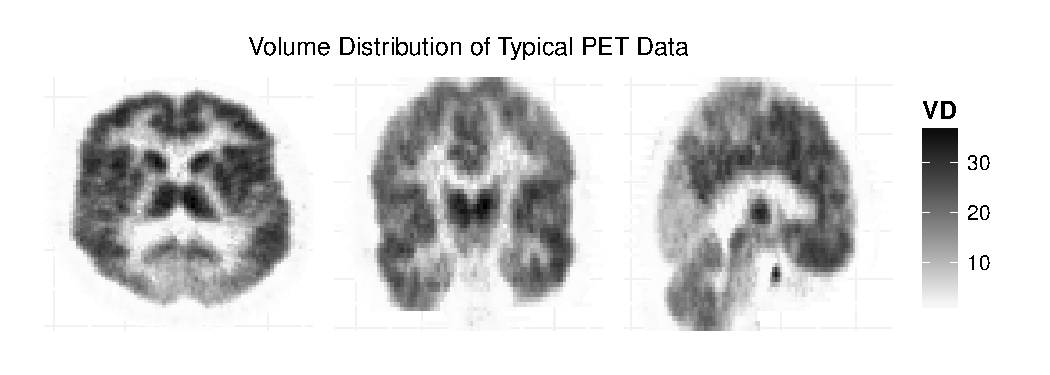
\includegraphics[width=\linewidth]{fig/PETPlot-smc2-ps-bw}
  \caption[Volume of distribution of real \protect\pet compartmental model
  data]
  {Estimates of $V_D$ from a single \pet scan as found using \smc[2].
    The data shows that the volume of distribution exhibits substantial
    spatial variation. Note that each pixel in the image represent an estimate
    from an individual time series data set. There are approximately a quarter
    of a million of them and each requires a Monte Carlo simulation to select
    a model.}
  \label{fig:petplot}
\end{figure}

As mentioned before, real neuroscience data sets involve a very large number
($\sim$200,000 per brain) of time series, which are typically somewhat
heterogeneous (also see Figure~\ref{fig:typical real pet}).
Figure~\ref{fig:petplot} shows estimates of $V_D$ from a typical \pet scan
generated using the \smc[2] algorithm as will be discussed later. Robustness
is therefore especially important. An application-specific \mcmc algorithm was
developed for this problem in \cite{Zhou2013} and its results are shown in the
Section~\ref{ssub:Generalized harmonic mean estimator}. A significant amount
of tuning of the algorithms was required to obtain good results.The results
shown in Figure~\ref{fig:petplot} are very close to those of \cite{Zhou2013}
but, as is shown later, they were obtained with almost no manual tuning effort
and at similar computational cost.

For the \smc and the population \mcmc algorithms, the requirement of
robustness means that the algorithm must be able to calibrate itself
automatically to different data (and thus different posterior surfaces). A
sequence of distributions which performs well for one time series may not
perform even adequately for another series. Specification of proposal scales
that produces fast-mixing kernels for one data series may lead to slow mixing
for another (as we already see in Section~\ref{sub:Adaptive specification of
  proposals}.) In the following experiment, we will use the simulated data
sets, and choose schedules that perform both well and poorly for this
particular time series.  The objective is to see if the algorithm can recover
from a relatively poorly specified schedule and obtain reasonably accurate
results.

\subsubsection{Results}

In this example we focus on the comparison between \smc[2] and population
\mcmc. We also consider parallelized implementations of algorithms. In this
case, due to its relatively small number of chains, population \mcmc can be
parallelized completely (and often cannot fully utilize the hardware
capability if a na\"\i ve approach to parallelization is taken; while we
appreciate that more sophisticated parallelization strategies are possible,
these depend intrinsically upon the model under investigation and the hardware
employed and given our focus on automatic and general algorithms, we don't
consider such strategies here.) The population \mcmc algorithm under this
setting is implemented such that each chain is updated at each iteration.
Further, for the \smc algorithms, we consider two cases. In the first we can
parallelize the algorithm completely (in the sense that each core has a single
particle associated with it.) In this setting we use a relatively small number
of particles and a larger number of time steps. In the second, we need a few
passes to process a large number of particles at each time step, and
accordingly we use fewer time steps to maintain the same total computation
time. These two settings allow us to investigate the trade-off between the
number of particles and time steps. In both implementations, we consider three
schedules, $\alpha(t/T) = t/T$ (linear), $\alpha(t/T) = (t/T)^5$ (prior), and
$\alpha(t/T) = 1 - (1 - t/T)^5$ (posterior). In addition, the adaptive
schedule based upon \cess is also implemented for the \smc[2] algorithm.

Results from 100 replicate runs of the two algorithms under various regimes
can be found in Table~\ref{tab:pet-py} and~\ref{tab:pet-bf} for the marginal
likelihood and Bayes factor estimates, respectively. The \smc algorithms
consistently outperforms the population \mcmc algorithms in the parallel
settings. The Monte Carlo \sd of \smc algorithms is typically of the order of
one fifth of the corresponding estimates from population \mcmc in most
scenarios. In some settings with the smaller number of samples, the two
algorithms can be comparable. Also at the lowest computational costs, the
samplers with more time steps and fewer particles outperform those with the
converse configuration by a fairly large margin in terms of estimator
variance. It shows that with limited resources, ensuring the similarity of
consecutive distributions, and thus good mixing, can be more beneficial than a
larger number of particles. However, when the computational budget is
increased, the difference becomes negligible.

\begin{table}
  \def\B{\color{MBlue}\it}
  \def\R{\color{MRed}\bf}
  \begingroup\small
    \begin{tabularx}{\linewidth}{lllCCCC}
      \toprule
      \multicolumn{3}{l}{Proposal scales}  & \multicolumn{3}{c}{Manual} & Adaptive \\
      \cmidrule(lr){1-3}\cmidrule(lr){4-6}\cmidrule(lr){7-7}
      \multicolumn{3}{l}{Annealing scheme} & Prior (5) & Posterior (5) & \multicolumn{2}{c}{Adaptive} \\
      \cmidrule(lr){1-3}\cmidrule(lr){4-4}\cmidrule(lr){5-5}\cmidrule(lr){6-7}
      %
      $T$    & $N$   & Algorithm   & \multicolumn{4}{c}{Marginal likelihood estimates ($\log p(\paramk|\data)\pm\text{\sd}$)} \\ \midrule
      $500$  & $30 $ & \pmcmc      & $ -39.1\pm  0.56$ & $-926.8\pm376.99$ && \\
      $500$  & $192$ & \smc2-\ds & $\B-39.2\pm0.25$ & $\B-39.7\pm1.06$ & $\B-39.2\pm0.18$ & $\R-39.1\pm0.12$ \\
             &       & \smc2-\ps & $\B-39.2\pm0.25$ & $-91.3\pm21.69$  & $\B-39.2\pm0.18$ & $-39.1\pm0.13$   \\
      $100 $ & $960$ & \smc2-\ds & $-39.3\pm0.36$   & $-40.6\pm1.41$   & $-39.2\pm0.31$   & $-39.2\pm0.19$   \\
             &       & \smc2-\ps & $-39.3\pm0.35$   & $302.1\pm46.29$  & $-39.3\pm0.31$   & $-39.2\pm0.18$   \\ \midrule
      $1000$ & $30 $ & \pmcmc      & $ -39.3\pm  0.46$ & $-884.1\pm307.88$ && \\
      $1000$ & $192$ & \smc2-\ds & $\B-39.2\pm0.19$ & $\B-39.4\pm0.68$ & $\B-39.2\pm0.17$ & $\R-39.1\pm0.10$ \\
             &       & \smc2-\ps & $\B-39.2\pm0.19$ & $-66.0\pm13.26$  & $\B-39.2\pm0.17$ & $\R-39.1\pm0.10$  \\
      $200 $ & $960$ & \smc2-\ds & $-39.2\pm0.22$   & $-39.8\pm1.21$   & $-39.2\pm0.18$   & $-39.1\pm0.11$   \\
             &       & \smc2-\ps & $-39.2\pm0.22$   & $175.5\pm26.84$  & $-39.2\pm0.18$   & $-39.2\pm0.11$   \\ \midrule
      $2000$ & $30 $ & \pmcmc      & $ -39.3\pm  0.28$ & $-928.7\pm204.93$ && \\
      $2000$ & $192$ & \smc2-\ds & $-39.2\pm0.14$   & $\B-39.3\pm0.41$ & $-39.1\pm0.12$   & $-39.1\pm0.07$  \\
             &       & \smc2-\ps & $-39.2\pm0.14$   & $-51.2\pm4.30$   & $-39.2\pm0.12$   & $-39.1\pm0.07$  \\
      $400 $ & $960$ & \smc2-\ds & $\B-39.2\pm0.13$ & $-39.4\pm0.73$   & $\B-39.2\pm0.11$ & $-39.2\pm0.07$   \\
             &       & \smc2-\ps & $\B-39.2\pm0.13$ & $106.0\pm14.36$  & $\B-39.2\pm0.11$ & $\R-39.2\pm0.06$ \\ \midrule
      $5000$ & $30$  & \pmcmc      & $ -39.3\pm  0.21$ & $-917.6\pm129.54$ && \\
      $5000$ & $192$ & \smc2-\ds & $-39.2\pm0.09$   & $\B-39.2\pm0.20$ & $-39.2\pm0.08$   & $-39.1\pm0.04$   \\
             &       & \smc2-\ps & $-39.2\pm0.09$   & $-43.8\pm2.13$   & $-39.2\pm0.08$   & $-39.1\pm0.04$   \\
      $1000$ & $960$ & \smc2-\ds & $\B-39.2\pm0.08$ & $-39.2\pm0.31$   & $\B-39.2\pm0.07$ & $\R-39.2\pm0.03$ \\
             &       & \smc2-\ps & $\B-39.2\pm0.08$ & $-65.7\pm5.54$   & $\B-39.2\pm0.07$ & $\R-39.2\pm0.03$ \\
      \bottomrule
    \end{tabularx}
  \endgroup
  \caption{Marginal likelihood estimates of two components \pet model. $T$:
    Number of distributions in \smc and number of iterations used for
    inference in \pmcmc. $N$: Number of particles in \smc and number chains in
    \pmcmc. The \pmcmc and \smc with $N = 192$ are completely $N$-way
    parallelized.  \smc with $N = 960$ are $N/5$-way parallelized. {\B
      Italic}: Minimum variance for the same computational cost and the same proposal
    scales and annealing schemes.  {\R Bold}: Minimum variance for the same computaitonal
    cost and all proposal scales and annealing schemes.}
  \label{tab:pet-py}
\end{table}

% & & $ -39.1\pm  0.56$ & $-926.8\pm376.99$ &&& \\
% & $\B-39.2\pm0.25$ & $\B-39.7\pm1.06$ & $\B-39.2\pm0.18$ & $\R-39.1\pm0.12$ & $\B-39.2\pm0.13$ \\
% & $\B-39.2\pm0.25$ & $-91.3\pm21.69$  & $\B-39.2\pm0.18$ & $-39.1\pm0.13$   & $\B-39.2\pm0.13$ \\
% & $-39.3\pm0.36$   & $-40.6\pm1.41$   & $-39.2\pm0.31$   & $-39.2\pm0.19$   & $-39.2\pm0.18$ \\
% & $-39.3\pm0.35$   & $302.1\pm46.29$  & $-39.3\pm0.31$   & $-39.2\pm0.18$   & $-39.2\pm0.19$ \\ \midrule
% & & $ -39.3\pm  0.46$ & $-884.1\pm307.88$ &&& \\
% & $\B-39.2\pm0.19$ & $\B-39.4\pm0.68$ & $\B-39.2\pm0.17$ & $\R-39.1\pm0.10$ & $-39.2\pm0.11$ \\
% & $\B-39.2\pm0.19$ & $-66.0\pm13.26$  & $\B-39.2\pm0.17$ & $\R-39.1\pm0.10$ & $\R-39.2\pm0.10$ \\
% & $-39.2\pm0.22$   & $-39.8\pm1.21$   & $-39.2\pm0.18$   & $-39.1\pm0.11$   & $-39.2\pm0.11$ \\
% & $-39.2\pm0.22$   & $175.5\pm26.84$  & $-39.2\pm0.18$   & $-39.2\pm0.11$   & $-39.2\pm0.12$ \\ \midrule
% & & $ -39.3\pm  0.28$ & $-928.7\pm204.93$ &&& \\
% & $-39.2\pm0.14$   & $\B-39.3\pm0.41$ & $-39.1\pm0.12$   & $-39.1\pm0.07$   & $\B-39.2\pm0.07$ \\
% & $-39.2\pm0.14$   & $-51.2\pm4.30$   & $-39.2\pm0.12$   & $-39.1\pm0.07$   & $\B-39.2\pm0.07$ \\
% & $\B-39.2\pm0.13$ & $-39.4\pm0.73$   & $\B-39.2\pm0.11$ & $-39.2\pm0.07$   & $-39.2\pm0.08$ \\
% & $\B-39.2\pm0.13$ & $106.0\pm14.36$  & $\B-39.2\pm0.11$ & $\R-39.2\pm0.06$ & $-39.2\pm0.08$ \\ \midrule
% & & $ -39.3\pm  0.21$ & $-917.6\pm129.54$ &&& \\
% & $-39.2\pm0.09$   & $\B-39.2\pm0.20$ & $-39.2\pm0.08$   & $-39.1\pm0.04$   & $-39.1\pm0.05$ \\
% & $-39.2\pm0.09$   & $-43.8\pm2.13$   & $-39.2\pm0.08$   & $-39.1\pm0.04$   & $-39.1\pm0.04$ \\
% & $\B-39.2\pm0.08$ & $-39.2\pm0.31$   & $\B-39.2\pm0.07$ & $\R-39.2\pm0.03$ & $-39.2\pm0.06$ \\
% & $\B-39.2\pm0.08$ & $-65.7\pm5.54$   & $\B-39.2\pm0.07$ & $\R-39.2\pm0.03$ & $\B-39.2\pm0.04$ \\

\thispagestyle{empty}
\newgeometry{hmargin={1in,1in},vmargin={1in,2in},bindingoffset=\mclassbinding}
\begin{table}[t]
  \linespread{1.1}\selectfont
  \caption[\protect\pet compartmental model Bayes factor estimates]
  {Bayes factor $B_{2,1}$ estimates of two components \pet model.} 
  \label{tab:pet-bf}
  \begin{tabu}{X[0.4l]X[0.4l]X[0.7c]X[0.8r]X[1r]X[0.8r]X[0.8r]}
      \toprule
      \multicolumn{3}{l}{Proposal scales}  & \multicolumn{3}{c}{Manual} & Adaptive \\
      \cmidrule(lr){1-3}\cmidrule(lr){4-6}\cmidrule(lr){7-7}
      \multicolumn{3}{l}{Annealing scheme} & Prior (5) & Posterior (5) & \multicolumn{2}{c}{Adaptive} \\
      \cmidrule(lr){1-3}\cmidrule(lr){4-4}\cmidrule(lr){5-5}\cmidrule(lr){6-7}
      %
      $T$    & $N$   & Algorithm   & \multicolumn{4}{c}{Bayes factor estimates ($\log B_{2,1}\pm\text{\sd}$)} \\ \midrule
      $500$  & $30 $ & \pmcmc      & $1.7\pm0.62$ & $-70.9\pm525.79$ && \\
      $500$  & $192$ & \smc2-\ds & $\SubBest{1.6\pm0.27}$ & $\SubBest{1.3\pm1.13}$  & $\SubBest{1.6\pm0.20}$ & $\Best{1.6\pm0.15}$  \\
             &       & \smc2-\ps & $\SubBest{1.6\pm0.27}$ & $-3.9\pm30.02$  & $\SubBest{1.6\pm0.20}$ & $\Best{1.6\pm0.15}$  \\
      $100 $ & $960$ & \smc2-\ds & $1.6\pm0.37$   & $0.5\pm1.55$    & $1.6\pm0.34$   & $1.6\pm0.21$    \\
             &       & \smc2-\ps & $1.6\pm0.37$   & $-13.1\pm66.30$ & $1.6\pm0.33$   & $1.6\pm0.21$    \\ \midrule
      $1000$ & $30 $ & \pmcmc      & $1.6\pm0.49$ & $-67.3\pm400.21$ && \\
      $1000$ & $192$ & \smc2-\ds & $\SubBest{1.6\pm0.21}$ & $\SubBest{1.5\pm0.79}$  & $1.6\pm0.20$   & $1.6\pm0.13$   \\
             &       & \smc2-\ps & $\SubBest{1.6\pm0.21}$ & $-0.6\pm15.47$  & $1.6\pm0.20$   & $1.6\pm0.13$   \\
      $200 $ & $960$ & \smc2-\ds & $1.6\pm0.25$   & $1.1\pm1.25$    & $1.6\pm0.19$   & $1.6\pm0.12$   \\
             &       & \smc2-\ps & $1.6\pm0.24$   & $-11.7\pm34.68$ & $\SubBest{1.6\pm0.18}$ & $\Best{1.6\pm0.11}$ \\ \midrule
      $2000$ & $30 $ & \pmcmc      & $1.6\pm0.31$ & $-95.5\pm264.74$ && \\
      $2000$ & $192$ & \smc2-\ds & $\SubBest{1.6\pm0.14}$ & $\SubBest{1.6\pm0.44}$  & $1.6\pm0.13$   & $1.6\pm0.09$    \\
             &       & \smc2-\ps & $\SubBest{1.6\pm0.14}$ & $1.6\pm6.06$    & $1.6\pm0.13$   & $1.7\pm0.09$    \\
      $400 $ & $960$ & \smc2-\ds & $1.6\pm0.16$   & $1.5\pm0.74$    & $\SubBest{1.6\pm0.12}$ & $\Best{1.6\pm0.08}$  \\
             &       & \smc2-\ps & $1.6\pm0.16$   & $-4.2\pm17.15$  & $\SubBest{1.6\pm0.12}$ & $\Best{1.6\pm0.08}$  \\ \midrule
      $5000$ & $30$  & \pmcmc      & $1.6\pm0.24$ & $-60.3\pm198.10$ && \\
      $5000$ & $192$ & \smc2-\ds & $1.6\pm0.10$   & $\SubBest{1.6\pm0.23}$  & $1.6\pm0.09$   & $1.6\pm0.05$    \\
             &       & \smc2-\ps & $1.6\pm0.10$   & $1.3\pm2.98$    & $1.6\pm0.09$   & $1.6\pm0.05$    \\
      $1000$ & $960$ & \smc2-\ds & $\SubBest{1.6\pm0.09}$ & $1.6\pm0.33$    & $\SubBest{1.6\pm0.08}$ & $\Best{1.6\pm0.04}$  \\
             &       & \smc2-\ps & $\SubBest{1.6\pm0.09}$ & $-0.2\pm6.63$   & $\SubBest{1.6\pm0.08}$ & $\Best{1.6\pm0.04}$  \\
      \bottomrule
    \multicolumn{7}{r}{%
      \begin{minipage}{\linewidth-2em}\vskip1ex\sffamily
        $T$: The number of distributions.

        $N$: The number of particles.

        Proposal: The proposal scales of the \mcmc kernels.

        Annealing: The annealing scheme of the distributions,
        $\alpha_k(t/T_k)$ in Equation~\ref{eq:geometry_2}.

        \Best: The estimate with the smallest variance among all algorithms
        settings.

        \SubBest: The estimate with the smallest variance for a single
        algorithm (\smc[2] or \pmcmc) among different settings.
      \end{minipage}}
    \end{tabu}
\end{table}
\restoregeometry

% & $1.7\pm0.62$ & $-70.9\pm525.79$ &&& \\
% & $\B1.6\pm0.27$ & $\B1.3\pm1.13$  & $\B1.6\pm0.20$ & $\R1.6\pm0.15$ & $\B1.6\pm0.16$ \\
% & $\B1.6\pm0.27$ & $-3.9\pm30.02$  & $\B1.6\pm0.20$ & $\R1.6\pm0.15$ & $\B1.6\pm0.16$ \\
% & $1.6\pm0.37$   & $0.5\pm1.55$    & $1.6\pm0.34$   & $1.6\pm0.21$   & $1.6\pm0.17$ \\
% & $1.6\pm0.37$   & $-13.1\pm66.30$ & $1.6\pm0.33$   & $1.6\pm0.21$   & $1.6\pm0.17$ \\ \midrule
% & $1.6\pm0.49$ & $-67.3\pm400.21$ &&& \\
% & $\B1.6\pm0.21$ & $\B1.5\pm0.79$  & $1.6\pm0.20$   & $1.6\pm0.13$   & $1.6\pm0.14$ \\
% & $\B1.6\pm0.21$ & $-0.6\pm15.47$  & $1.6\pm0.20$   & $1.6\pm0.13$   & $1.6\pm0.13$ \\
% & $1.6\pm0.25$   & $1.1\pm1.25$    & $1.6\pm0.19$   & $1.6\pm0.12$   & $1.6\pm0.13$ \\
% & $1.6\pm0.24$   & $-11.7\pm34.68$ & $\B1.6\pm0.18$ & $\R1.6\pm0.11$ & $\B1.6\pm0.12$ \\ \midrule
% & $1.6\pm0.31$ & $-95.5\pm264.74$ &&& \\
% & $\B1.6\pm0.14$ & $\B1.6\pm0.44$  & $1.6\pm0.13$   & $1.6\pm0.09$   & $1.6\pm0.11$ \\
% & $\B1.6\pm0.14$ & $1.6\pm6.06$    & $1.6\pm0.13$   & $1.7\pm0.09$   & $1.6\pm0.10$ \\
% & $1.6\pm0.16$   & $1.5\pm0.74$    & $\B1.6\pm0.12$ & $\R1.6\pm0.08$ & $\B1.6\pm0.09$ \\
% & $1.6\pm0.16$   & $-4.2\pm17.15$  & $\B1.6\pm0.12$ & $\R1.6\pm0.08$ & $\B1.6\pm0.09$ \\ \midrule
% & $1.6\pm0.24$ & $-60.3\pm198.10$ &&& \\
% & $1.6\pm0.10$   & $\B1.6\pm0.23$  & $1.6\pm0.09$   & $1.6\pm0.05$   & $1.6\pm0.06$ \\
% & $1.6\pm0.10$   & $1.3\pm2.98$    & $1.6\pm0.09$   & $1.6\pm0.05$   & $1.6\pm0.06$ \\
% & $\B1.6\pm0.09$ & $1.6\pm0.33$    & $\B1.6\pm0.08$ & $\R1.6\pm0.04$ & $1.6\pm0.06$ \\
% & $\B1.6\pm0.09$ & $-0.2\pm6.63$   & $\B1.6\pm0.08$ & $\R1.6\pm0.04$ & $\B1.6\pm0.05$ \\


\paragraph{Effects of adaptive schedule}

A set of samplers with adaptive schedules are also used. Due to the nature of
the schedule, it cannot be controlled to have exactly the same number of time
steps as non-adaptive procedures. However, the \cess was controlled such that
the average number of time steps are comparable with the fixed schedules and
in most cases slightly less than the fixed numbers.

It is found that, with little computational overhead, adaptive schedules do
provide the best results (or very nearly so) and do so without user
intervention. The reduction of Monte Carlo \sd varies among different
configurations. For moderate or larger number of distributions, a reduction
about 50\% was observed. In addition, it shall be noted that, in this example,
the bias of the path sampling estimates are much more sensitive to the
schedules than the previous Gaussian mixture model example. A vanilla linear
schedule does not provide a low bias estimator at all even when the number of
distributions is increased to a considerably larger number. The prior schedule
though provides a nearly unbiased estimator, there is no clear theoretical
evidence showing that this shall work for other situations. Even it has more
general usage, as suggested in \cite{Calderhead:2009bd}, the power still has
to be chosen (in the previous \gmm example, $p = 2$ was the best choice while
in this \pet example $p = 5$ is more suitable). In contrast, The adaptive
schedule, without any manual calibration, can provide a nearly unbiased
estimator, even when path-sampling is employed, in addition to potential
variance reduction.

\paragraph{Bias reduction for path sampling estimator}

\begin{table}[t]
  \linespread{1.1}\selectfont
  \caption{Path sampling estimates of marginal likelihood of two-compartments
    \protect\pet model for the simulated data set.}
  \label{tab:pet-bias}
  \begin{tabularx}{\linewidth}{lXXXX}
    \toprule
    & \multicolumn{4}{c}{Number of grid points (compared to sampled iterations)} \\
    \cmidrule(lr){2-5}
    Integration rule & $\times1$ & $\times2$ & $\times4$ & $\times8$ \\
    \midrule
    Trapezoid
    & $-52.2\pm5.01$ & $-45.5\pm1.93$ & $-42.1\pm1.21$ & $-40.5\pm1.06$ \\
    Simpson
    & $-43.2\pm1.39$ & $-41.0\pm1.10$ & $-40.0\pm1.04$ & $-39.4\pm1.04$ \\
    Simpson $3/8$
    & $-42.1\pm1.21$ & $-40.5\pm1.06$ & $-39.7\pm1.04$ & $-39.3\pm1.04$ \\
    Boole
    & $-40.9\pm1.09$ & $-39.9\pm1.04$ & $-39.4\pm1.04$ & $-39.2\pm1.05$ \\
    \bottomrule
    \multicolumn{5}{r}{%
      \begin{minipage}{\linewidth-2em}\vskip1ex\sffamily
        The estimator was approximated using samples from \smc[2] algorithm
        with 1,000 particles and 20 iterations, with different numerical
        integration strategies. Large sample result (see
        Table~\ref{tab:pet-py}) shows that the accurate value is about
        $-39.2$.
      \end{minipage}}
  \end{tabularx}
\end{table}


As seen in Table~\ref{tab:pet-py} and~\ref{tab:pet-bf}, a bad choice of
schedule $\alpha(t/T)$ can results in considerable bias for the basic path
sampling estimator, here for \smc[2]-\ps but the problem is independent of the
mechanism by which the samples are obtained. Increasing the number of
iterations can reduce this bias but at the cost of additional computation
time. As outlined in Section~\ref{sub:Improved univariate numerical
  integration}, in the case of the \smc algorithms discussed here, it is
possible to reduce the bias without increasing computational cost
significantly. To demonstrate the bias reduction effect, we constructed \smc
sampler for the above \pet example with only 1,000 particles and about 20
iterations specified using the \cess based adaptive strategy. The path
sampling estimator was approximated using Equation~\eqref{eq:path_est} as well
as other higher order numerical integration or by integrating over a grid that
contains $\{\alpha_t\}$ at which the samples was generated. The results are
shown in Table~\ref{tab:pet-bias}

\paragraph{Trade-off between number of particles and distributions}

\begin{figure}[t]
  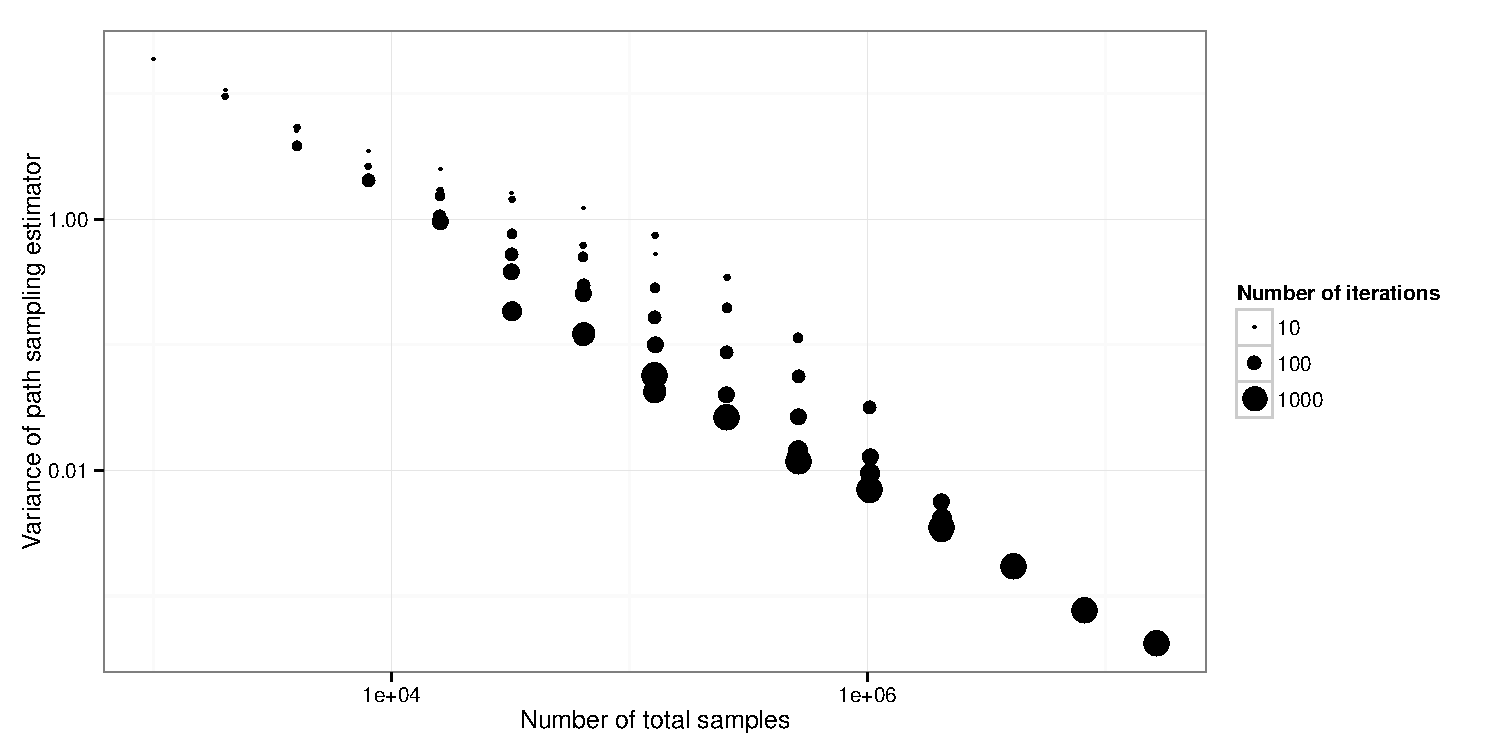
\includegraphics[width=\linewidth]{fig/Particle_Iter_Var}
  \caption[Variance of path sampling estimator and total number of samples
  using \protect\smc algorithm]
  {Variance of path sampling estimator and total number of samples
    using the \smc[2] algorithm.}
  \label{fig:particle iter num}
\end{figure}

It can be seen through the nonlinear \ode and the \pet examples that, there is
a trade-off between the number of particles and distributions. Increasing
either of them can improve the accuracy of estimates. We consider a range of
number of particles (from 100 to more than 10,000) and a range of number of
distributions using the prior schedule ($\alpha(t/T) = (t/T)^5$; from as small
as 10 to more than 1,000.) When applied to the simulated data sets, the
variance of the path sampling estimates is plotted against the total number of
samples (the product of these two quantities) in Figure~\ref{fig:particle iter
  num}. It can be seen that, for the same total number of samples, samplers
with larger number of distributions outperform those with larger number of
particles by a considerable large margin. However, as the number of samples
increase, the difference becomes smaller and smaller. This suggests that it
will be better to first allocate a fixed number of particles, according to
considerations such as computation hardwares. And then use the number of
distributions as a performance parameter to tune the sampler for desired
accuracy. When using the adaptive algorithms proposed in this work, it is
equivalent to tune the value of $\cess^\star$. As shown in
Section~\ref{sub:Adaptive specification of distributions}, the relation
between $\cess^\star$ and the variance of estimators provides a predictable
way to configure the samplers.

\paragraph{Fast mixing \mcmc kernels and number of distributions}

As mentioned in Section~\ref{sub:Optimal and suboptimal backward kernels}, the
suboptimal backward kernel and its associated incremental weights used in the
above examples could perform poorly if the adjacent distributions are not
close, even when the transition kernel mixes well. However, both fast mixing
kernels and more intermediate distributions (and thus a smoother sequence),
can improve the performance of the sampler. To improve the mixing speed of the
kernel, one can apply multiple passes of \mcmc moves at each iteration. Here
we compare two samplers use the simulated data sets, both with 1,000 particles.
One sampler use 10 \mcmc moves at each iteration. The other only use one \mcmc
move but use ten times the number of distributions. The annealing scheme, for
simplicity, is chosen to be $\alpha(t/T) = (t/T)^5$. The results of the path
sampling variance is shown in Figure~\ref{fig:fast mcmc iter}. It can be seen
that, given the same total number of samples simulated, using more
distributions almost always outperforms using more \mcmc moves. However, with
sufficient large number of samples, the difference is minimal.

\begin{figure}[t]
  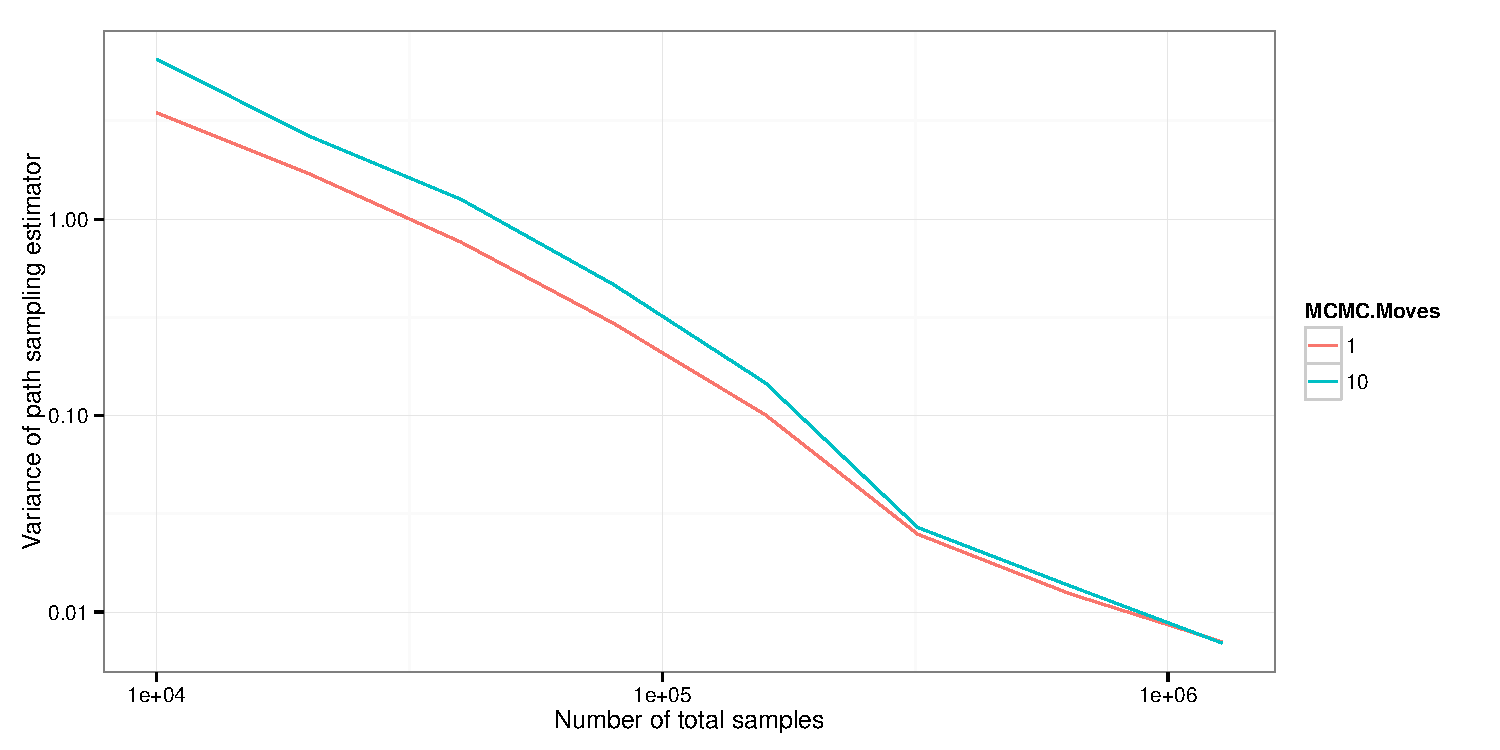
\includegraphics[width=\linewidth]{fig/MCMC_Iter_Var}
  \caption[Variance of path sampling estimator and total number of samples
  using \protect\smc algorithm]
  {Variance of path sampling estimates and total number of samples
    using the \smc[2] algorithm. Both samplers use 1,000 particles but with
    different number of distributions and passes of \mcmc moves at each
    iteration}
  \label{fig:fast mcmc iter}
\end{figure}

\paragraph{Real data results}

Finally, the methodology of \smc[2]-\ps was applied to measured positron
emission tomography data using the same compartmental setup as in the
simulations. The data shown in Figure~\ref{fig:petplot} comes from a study
into opioid receptor density in Epilepsy, with the data being described in
detail in \cite{Jiang:2009kf}. It is expected that there will be considerable
spatial smoothness to the estimates of the volume of distribution, as this is
in line with the biology of the system being somewhat regional. Some regions
will have much higher receptor density while others will be much lower,
yielding higher and lower values of the volume of distribution, respectively.
While we did not impose any spatial smoothness but rather estimated the
parameters independently for each time series at each spatial location, as can
be seen, smooth spatial estimates of the volume of distribution consistent
with neurological understanding were found using the approach. This method is
computationally feasible for the entire brain on a voxel-by-voxel basis, due
to the ease of parallelization of the \smc algorithm. In the analysis
performed here 1,000 particles were used, along with an adaptive schedule
using a constant $\cess^\star/N = 0.999$, resulting in about 180 to 200
intermediate distributions. The model selection results are very close to
those obtained by a  previous study of the same data \cite{Zhou2013}, although
the present approach requires much less implementation effort and has roughly
the same computational cost.

\subsection{Summary}

These three illustrative applications have essentially shown three aspects of
using \smc as a generic tool for Bayesian model selection. Firstly, as seen in
the Gaussian mixture model example, all the different variants of \smc
proposed, including both direct and path sampling versions, produce results
which are competitive with other model selection methods such as \rjmcmc and
population \mcmc. In addition, in this somewhat simple example, \smc[2]
performs well, and leads to low variance estimates with no appreciable bias.
The effect of adaptation was studied more carefully in the nonlinear \ode
example, and it was shown that using both adaptive selection of distributions
as well as adaptive proposal variances leads to very competitive algorithms,
even against those with significant manual tuning. This suggests that an
automatic process of model selection using \smc[2] is possible. In the final
example, considering the easy parallelization of algorithms such as \smc[2]
suggests that great gains in variance estimation can be made using settings
such as \gpu computing for application where computational resources are of
particular importance (such as in image analysis as in the PET example). It is
also clear that the negligible cost of the bias reduction techniques described
means that one should always consider using these to reduce the bias inherent
in path sampling estimation.

\section{Discussion}
\label{sec:Bayesian SMC discussion}

It has been shown that \smc is an effective Monte Carlo method for Bayesian
inference for the purpose of model comparison. Three approaches have been
outlined and investigated in several illustrative applications including the
challenging scenarios of nonlinear \ode models and \pet compartmental systems.
The proposed strategy is always competitive and often substantially
outperforms the state of the art in this area.

It has been demonstrated that it is possible to use the \smc algorithms to
estimate the model probabilities directly (\smc[1]), or through individual
model evidence (\smc[2]), or pair-wise relative evidence (\smc[3]). In
addition, both \smc[2] and \smc[3] algorithms can be coupled with the path
sampling estimator.

Among the three approaches, \smc[1] is applicable to very general settings. It
can provide a robust alternative to \rjmcmc when inference on a countable
collection of models is required (and could be readily combined with the
approach of \cite{Jasra:2008bb} at the expense of a little additional
implementation effort). However, like all Monte Carlo methods involving
between model moves, it can be difficult to design efficient algorithms in
practice. The \smc[3] algorithm is conceptually appealing. However, the
existence of a suitable sequence of distributions between two posterior
distributions may not be obvious.

The \smc[2] algorithm, which only involves within-model simulation, is most
straightforward to implement in many interesting problems. It has been shown
to be exceedingly robust in many settings. As it depends largely upon a
collection of within-model \mcmc moves, any existing \mcmc algorithms can be
reused in the \smc[2] framework. However, much less tuning is required because
the algorithm is fundamentally less sensitive to the mixing of the Markov
kernel and it is possible to implement effective adaptive strategies at little
computational cost. With adaptive placement of the intermediate distributions
and specification of the \mcmc kernel proposals, it provides a robust and
essentially automatic model comparison method.

Compared to the population \mcmc algorithm, \smc[2] has greater flexibility in
the specification of distributions. Unlike population \mcmc, where the number
and placement of distributions can affect the mixing speed and hence
performance considerably, increasing the number of distributions will always
benefit an \smc sampler given the same number of particles. When coupled with a
path sampling estimator, this leads to less bias and variance. Compared to its
no-resampling variant, it has been shown that \smc samplers with resampling
can reduce the variance of normalizing constant estimates considerably.

Even after three decades of intensive development, no Monte Carlo method can
solve the Bayesian model comparison problem completely automatically without
any manual tuning. However, \smc algorithms and the adaptive strategies
demonstrated in this paper show that even for realistic, interesting problems,
these samplers can provide good results with very minimal tuning and few
design difficulties. For many applications, they could already be used as near
automatic, robust solutions. For more challenging problems, the robustness of
the algorithms can serve as solid foundation for specific algorithm designs.
